
\documentclass[aspectratio=169,11pt]{beamer}

% --- Kodowanie i język ---
\usepackage[T1]{fontenc}
\usepackage[utf8]{inputenc}
\usepackage[english]{babel}

% --- Matematyka ---
\usepackage{amsmath}
\usepackage{amssymb}
\usepackage{mathtools}
\DeclareMathOperator*{\argmax}{arg\,max}

% --- Grafiki i tabele ---
\usepackage{graphicx}
\usepackage{booktabs}
\usepackage{array}

% --- Linki i kolory ---
\usepackage{hyperref}
\usepackage{xcolor}

% --- Motyw prezentacji ---
\usetheme{Madrid}
\usefonttheme{professionalfonts}
\usepackage{newtxtext}
\usepackage{newtxmath}

% Main accent color
\definecolor{myorange}{RGB}{199,101,36}
\definecolor{lightorange}{RGB}{250,237,225}

% General structure: bullets, markers, etc.
\setbeamercolor{structure}{fg=myorange}

% Block headers
\setbeamercolor{block title}{fg=white, bg=myorange}

% Block contents
\setbeamercolor{block body}{fg=black, bg=lightorange}

% Example blocks
\setbeamercolor{block title example}{fg=white, bg=myorange}
\setbeamercolor{block body example}{fg=black, bg=lightorange}

% Alert blocks
\setbeamercolor{block title alerted}{fg=white, bg=myorange}
\setbeamercolor{block body alerted}{fg=black, bg=lightorange}


% --- Dane prezentacji ---
\title{CFM}
\subtitle{Language-aligned Concept Foundation Model for Vision}
\author{Julia Borowska \& Mateusz Wątły}
\date{4 November 2026}

\begin{document}

% --- Slajd tytułowy ---
\begin{frame}
    \titlepage
\end{frame}

% -------------------------------------------------
\begin{frame}{The Problem: Explanations Can Be Misleading}
    \framesubtitle{Why do interpretable concepts need spatial grounding?}

    \centering
    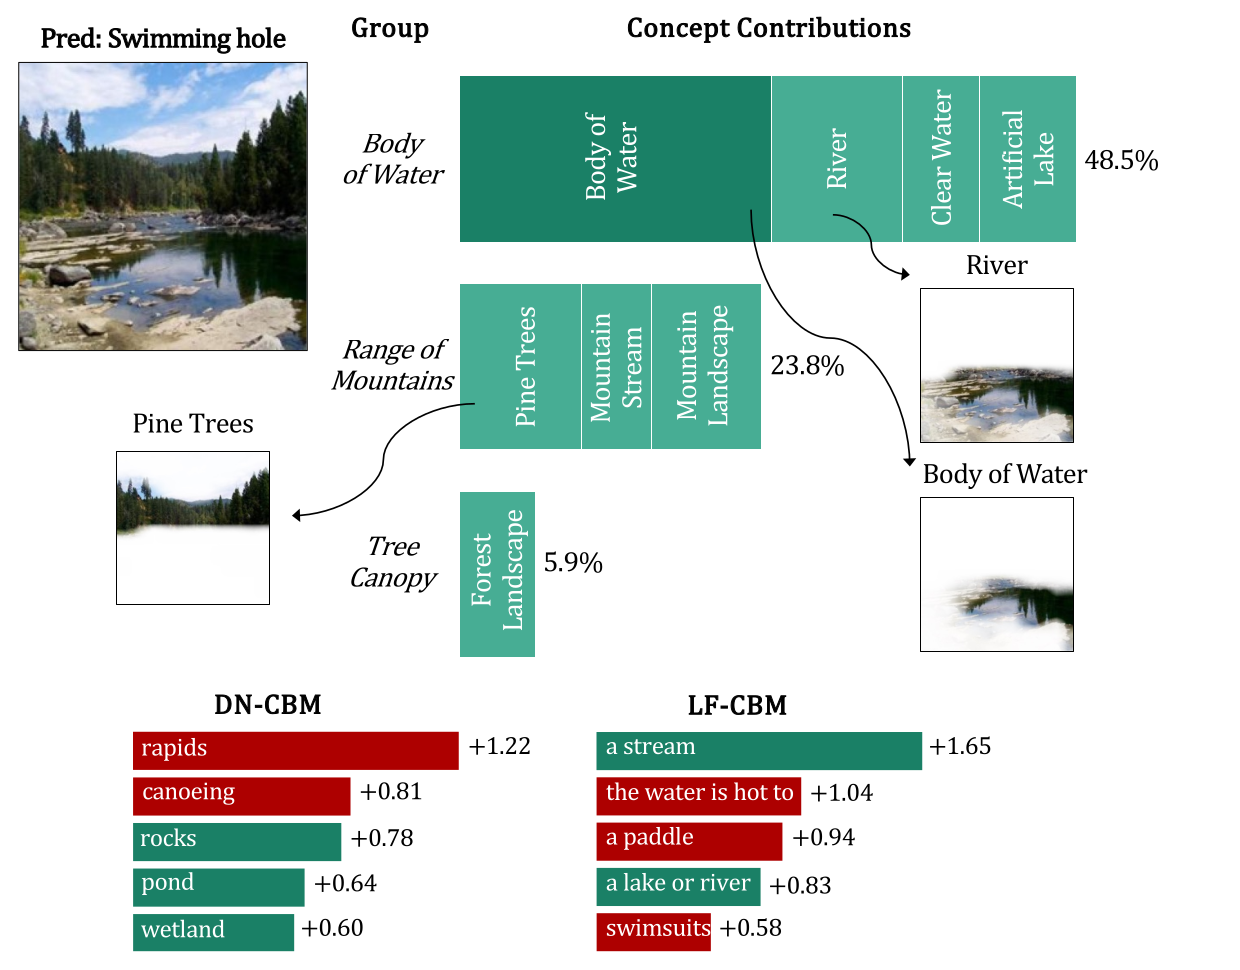
\includegraphics[
        width=0.88\textwidth,
        height=0.72\textheight,
        keepaspectratio,
        trim=0 43bp 0 0,
        clip
    ]{figure6_comparison.png}

    \vspace{0.06cm}

    {\footnotesize
    \textbf{Other models:}
    Absent concepts (\emph{canoeing}, \emph{swimsuits}).
    \qquad
    \textbf{CFM:}
    Concepts grounded in image regions.\par}

    \vspace{0.04cm}

    {\tiny Fig. 6 \par}
\end{frame}

% -------------------------------------------------
\begin{frame}{Why Do We Need CFM?}
    \framesubtitle{Bridging foundation models and interpretable concepts}

    \centering

    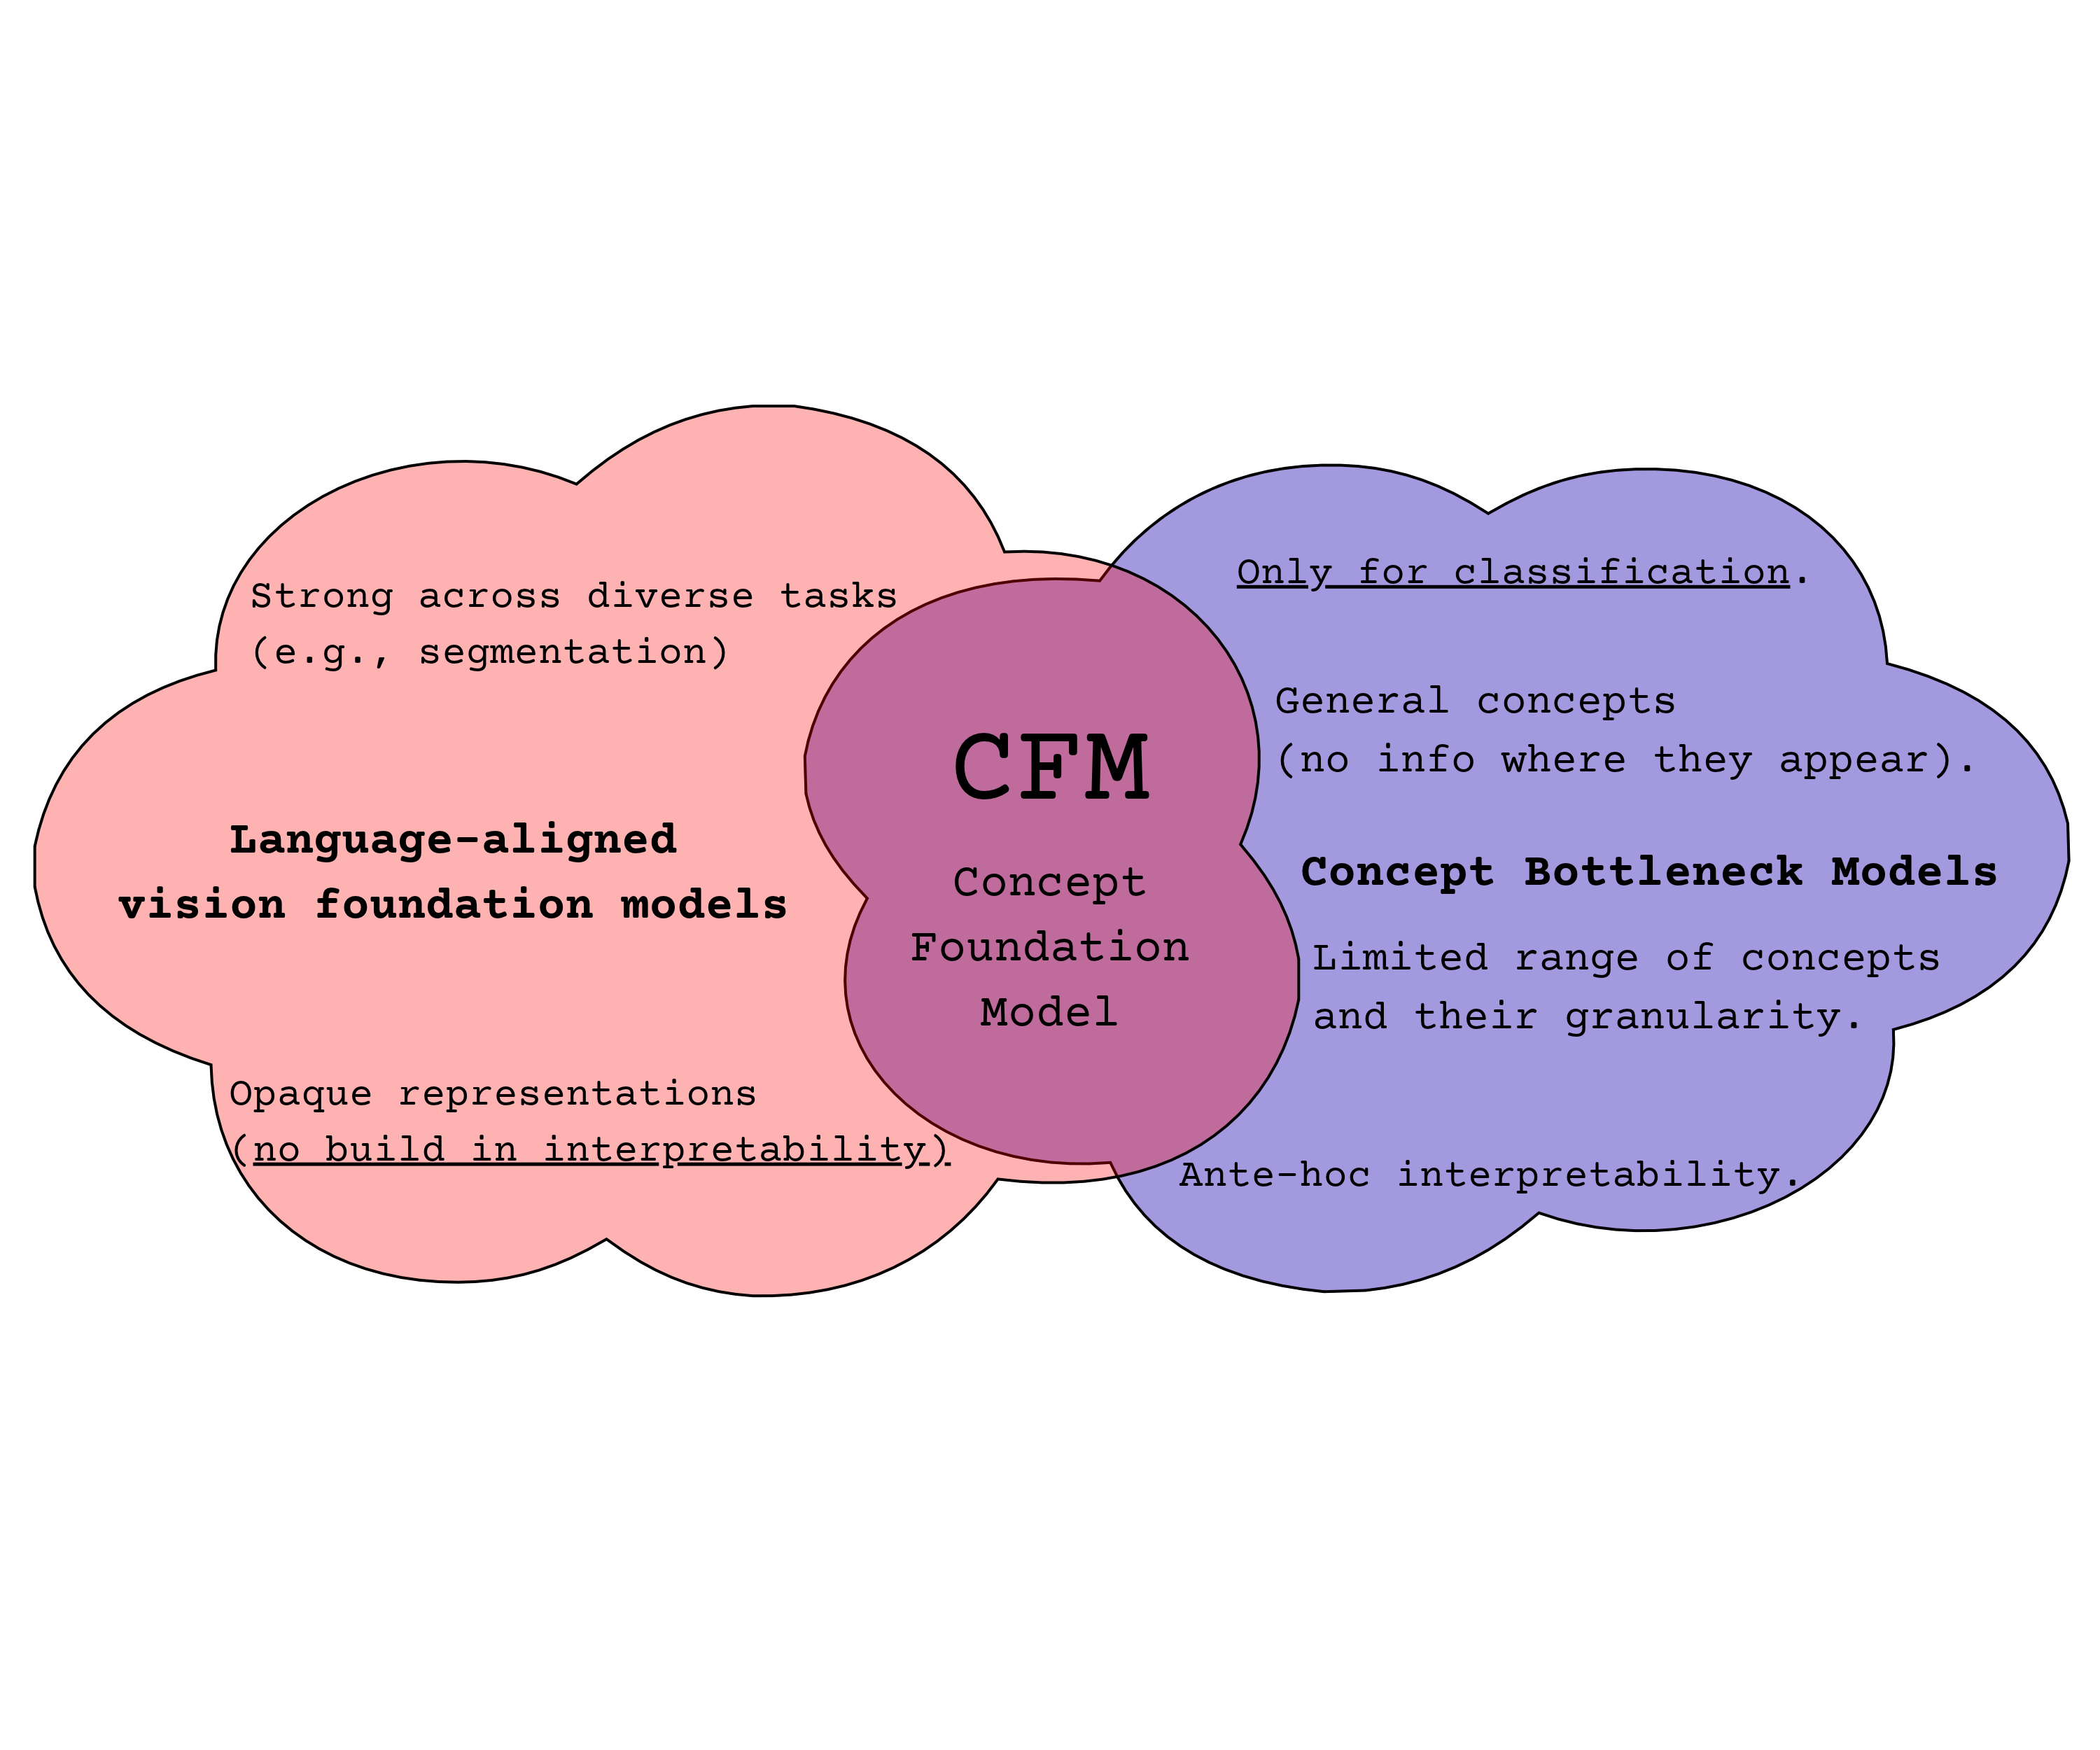
\includegraphics[
        width=0.96\textwidth,
        height=0.65\textheight,
        keepaspectratio,
        trim=32bp 440bp 28bp 394bp,
        clip
    ]{cfm_motivation.jpg}

    %\vspace{0.15cm}

    %\begin{block}{The Motivation}
    %    \small
    %    CFM aims to combine the broad capabilities of
    %    language-aligned vision models with the
    %    interpretability of concept-based models.
    %\end{block}

\end{frame}

% -------------------------------------------------
\begin{frame}{What Changes with CFM?}
    \framesubtitle{A reusable, spatially grounded concept representation}

    \vspace{-0.4em}
    \centering
    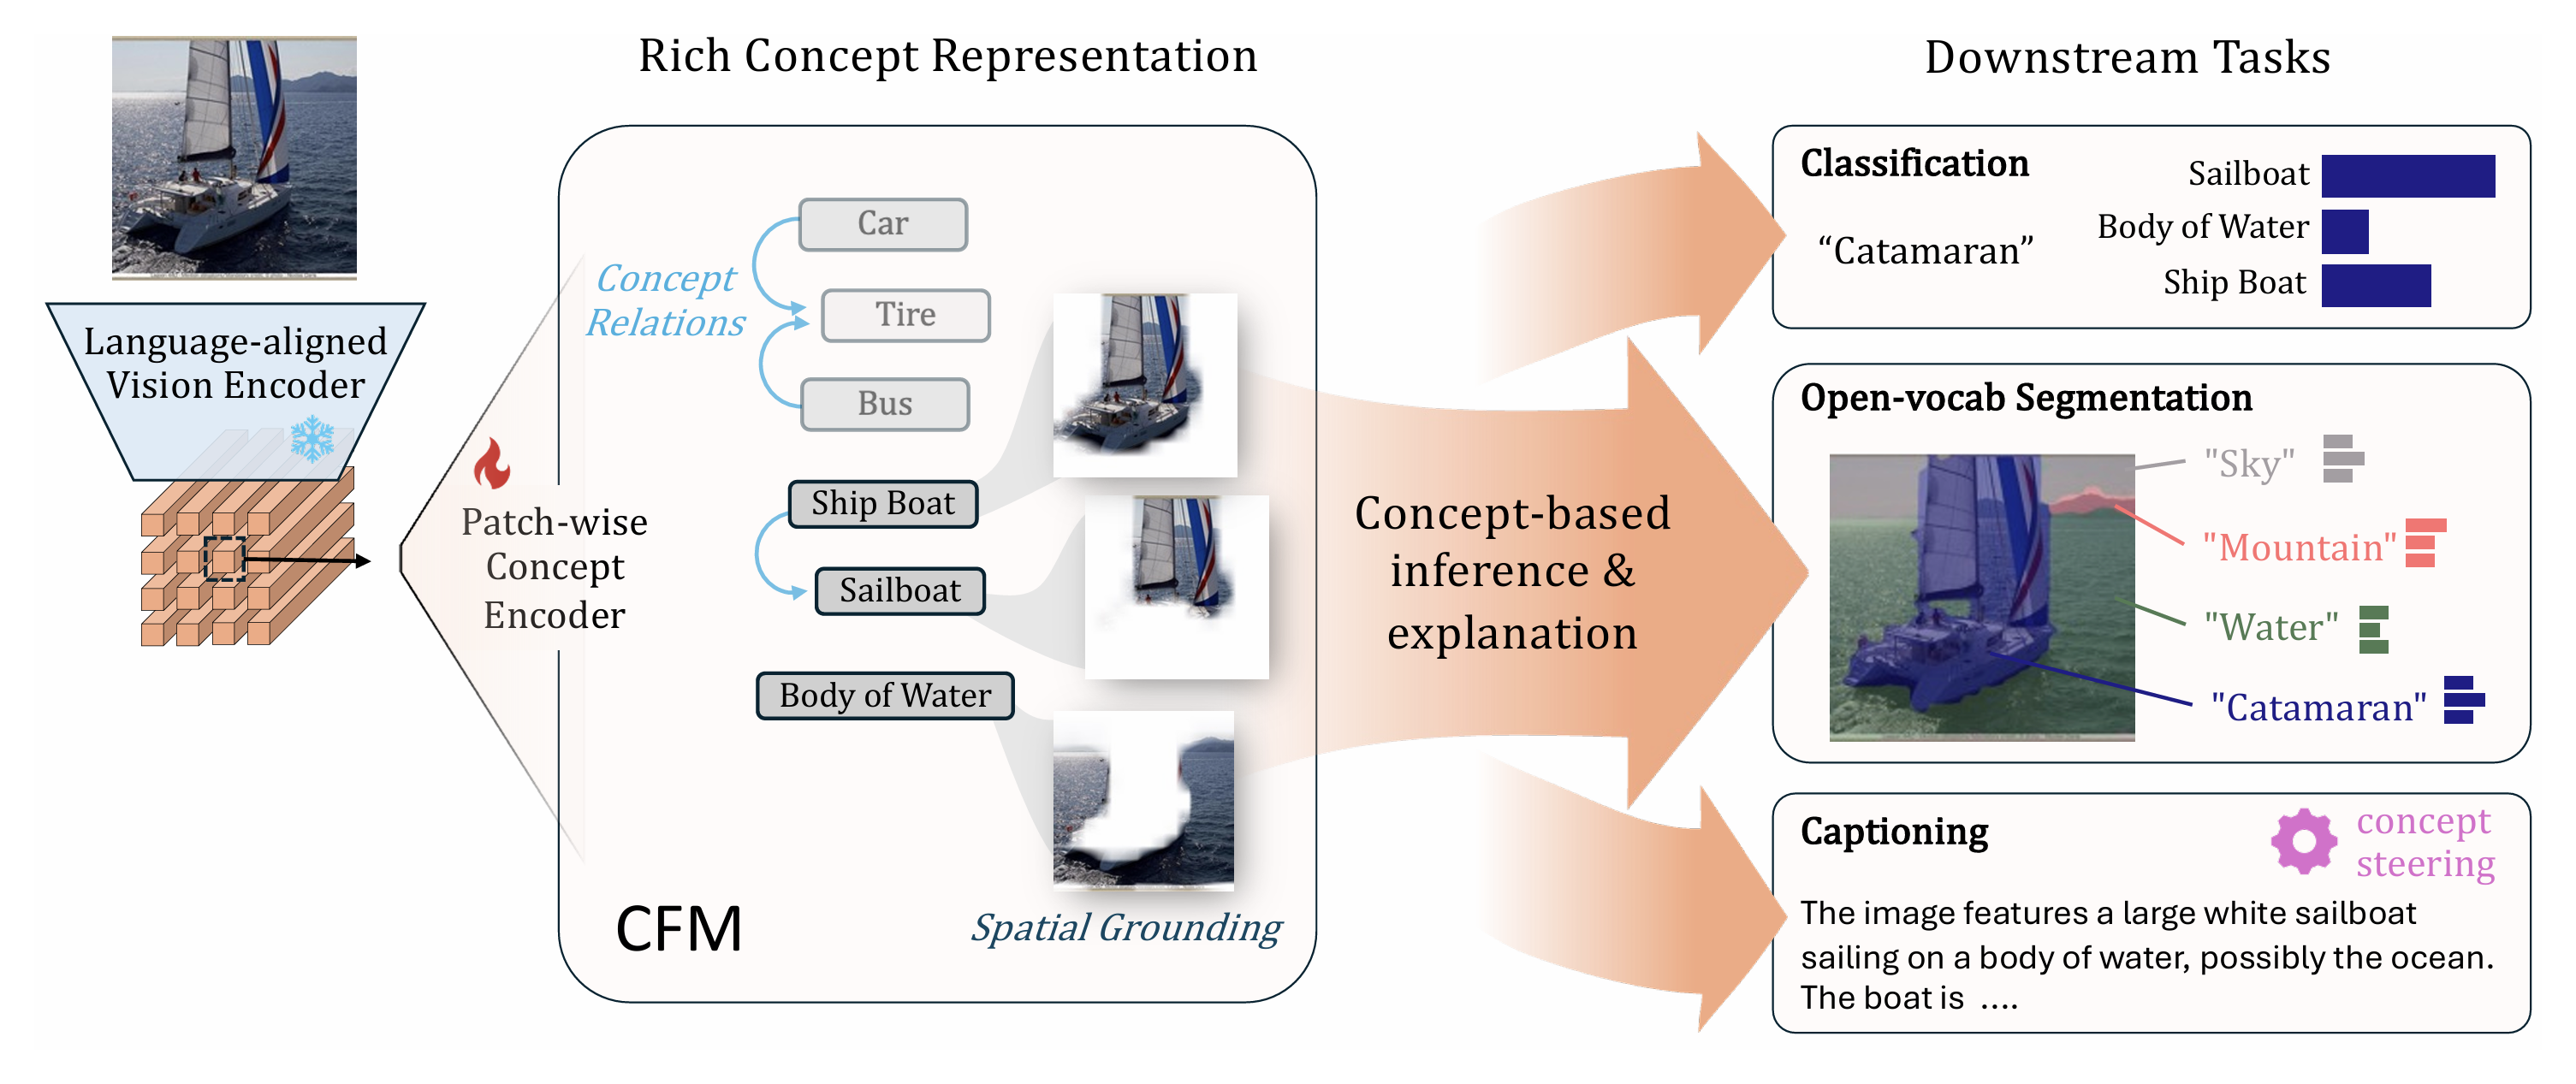
\includegraphics[
        width=\linewidth,
        height=0.58\textheight,
        keepaspectratio
    ]{figure1_overview.png}

    \vspace{-1.25em}
    {\tiny Fig. 1}

    \vspace{-1.05em}

    \begin{columns}[T,onlytextwidth]
        \begin{column}{0.48\textwidth}
            \begin{block}{\small Previous approaches}
                \scriptsize
                Mainly image-level concepts and
                classification-oriented explanations.
            \end{block}
        \end{column}

        \begin{column}{0.48\textwidth}
            \begin{block}{\small CFM}
                \scriptsize
                Spatially localized concepts with
                hierarchical relationships, reusable
                across different vision tasks.
            \end{block}
        \end{column}
    \end{columns}
\end{frame}

% -------------------------------------------------
\begin{frame}{Transparency of Model Predictions}
    \framesubtitle{Why does CFM matter for Trustworthy ML?}

    \begin{columns}[T,onlytextwidth]
        \begin{column}{0.71\textwidth}
            \centering
            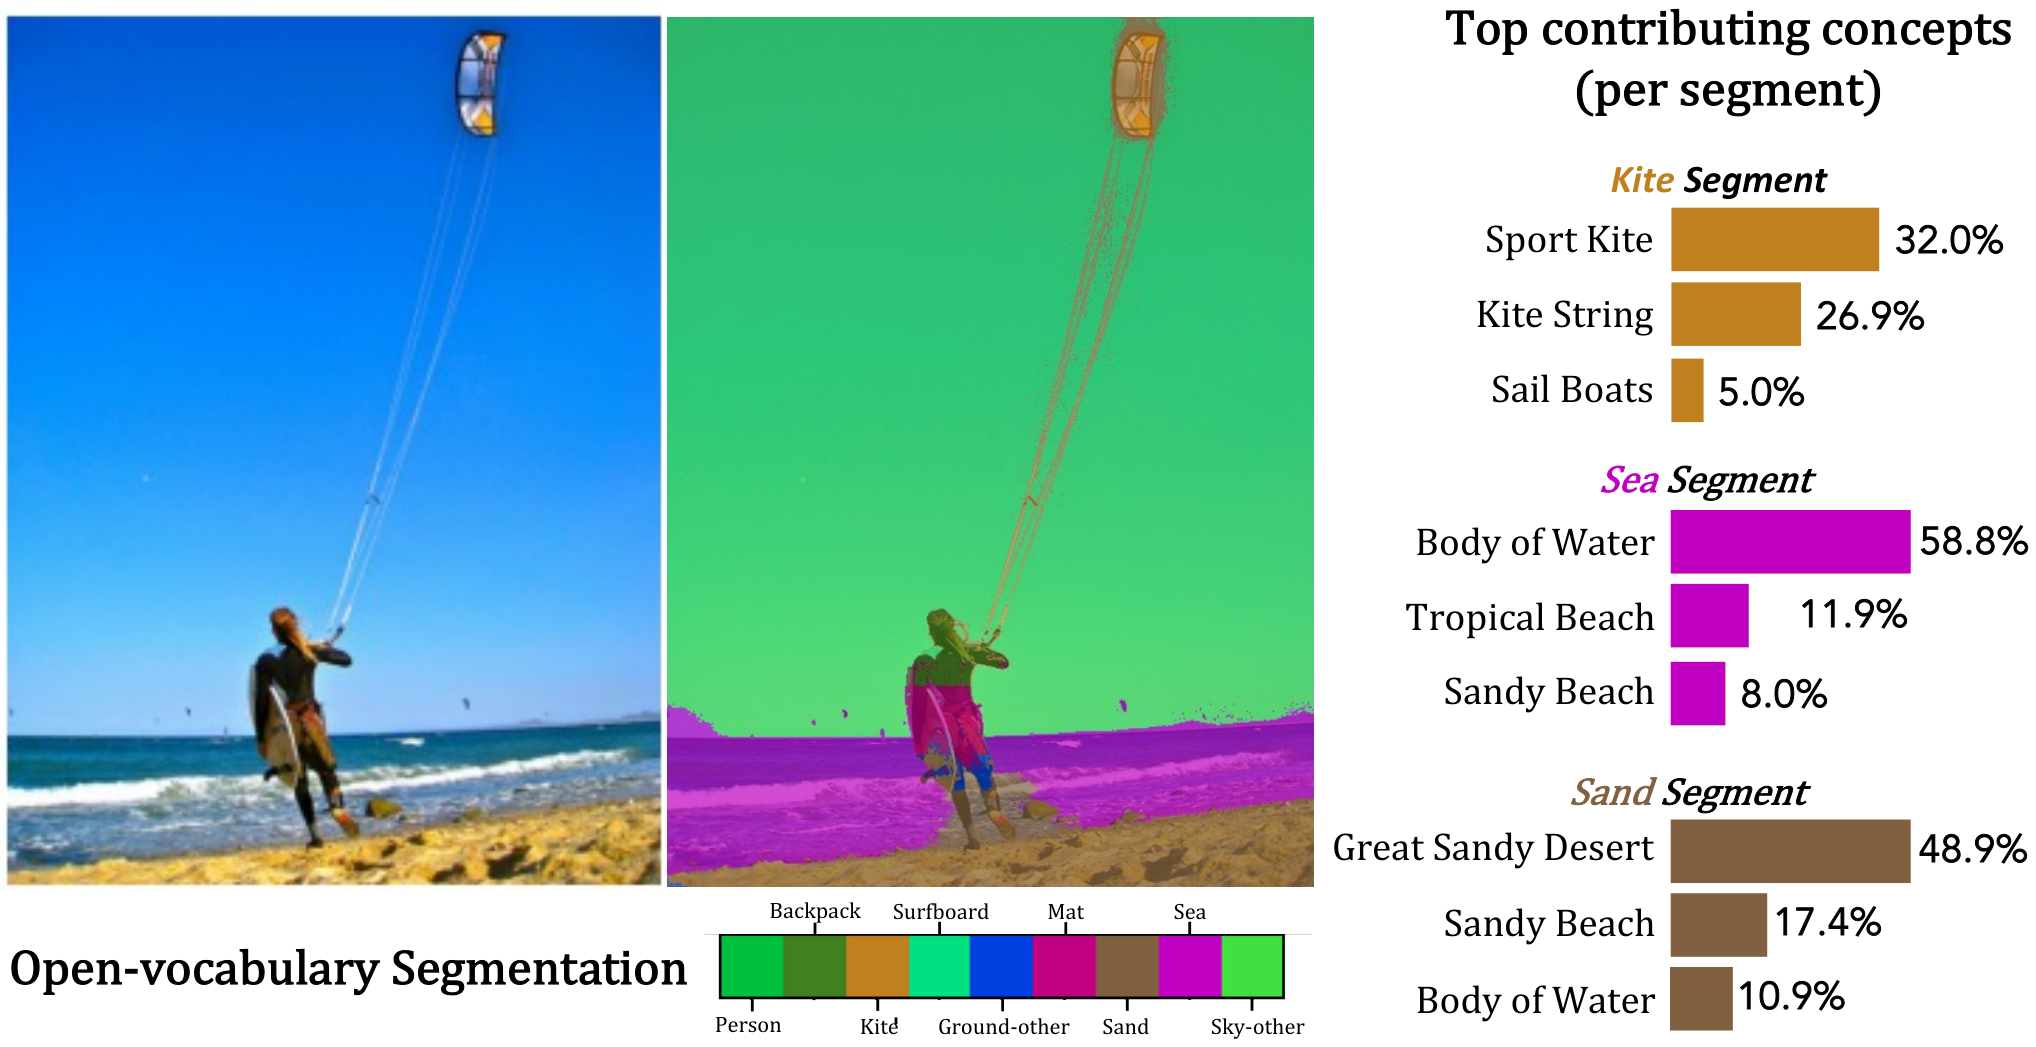
\includegraphics[
                width=\linewidth,
                height=0.77\textheight,
                keepaspectratio
            ]{figure8_segmentation.png}

            {\tiny Fig. 8}
        \end{column}

        \begin{column}{0.27\textwidth}
            \small
            \textbf{CFM provides:}
            \begin{itemize}
                \item Localized predictions.
                \item Concepts contributing to each prediction.
                \item Concept contribution scores.
            \end{itemize}

            \vspace{0.25cm}

            \textbf{Trustworthy ML:}
            \begin{itemize}
                \item Transparency
                \item Auditability
                \item Error analysis
            \end{itemize}
        \end{column}
    \end{columns}

    \vspace{0.15cm}
    \centering
    \footnotesize
    Interpretability facilitates model inspection,
    but does not guarantee correctness or robustness.
\end{frame}

% -------------------------------------------------
\begin{frame}{Contributions}
    \begin{columns}[onlytextwidth]
        % Left column
        \begin{column}{0.48\textwidth}
            \begin{block}{\small CFM provides concepts that are:}
                \begin{itemize}
                    \small
                    \item \textbf{Fine-grained:} at different levels of detail
                    \item \textbf{Spatially grounded:} well localized in the image
                    \item \textbf{Unified:} shared across different downstream tasks
                \end{itemize}
            \end{block}
            % \vspace{0.5cm}
            \uncover<2->{
            \begin{block}{\small CFM automatically discovers concept relations:}
                \begin{itemize}
                    \small
                    \item \textbf{Based on local co-occurrences:} concepts activated in the same image regions
                    \item \textbf{Specifications:} e.g. \textit{turtle} → \textit{leatherback turtle}
                    \item \textbf{Part-relations:} e.g. \textit{turtle} → \textit{turtle shell}
                \end{itemize}
            \end{block}
            }
        \end{column}

        % Right column
        \begin{column}{0.48\textwidth}
            \uncover<3->{
            \begin{block}{\small CFM improves concept labeling by:}
                \begin{itemize}
                    \small
                    \item \textbf{Matching concepts with text labels} from a large vocabulary
                    \item Taking \textbf{concept hierarchies} into account
                    \item Using \textbf{parent concepts} to better identify \textbf{specific concepts}
                \end{itemize}
            \end{block}
            }
            % \vspace{0.5cm}
            \uncover<4->{
            \begin{block}{\small CFM provides:}
                \begin{itemize}
                    \small
                    \item \textbf{Human-interpretable explanations}
                    \item \textbf{Competitive performance} in classification, segmentation, and captioning
                    \item \textbf{Steerable outputs} through concept representations
                \end{itemize}
            \end{block}
            }
        \end{column}
    \end{columns} 
\end{frame}

% -------------------------------------------------
\begin{frame}
\begin{center}
    \begin{minipage}{0.6\textwidth}
        \begin{block} {\centering \huge CFM Method}
            \begin{itemize}
                \item Extracting Concept Representations
                \item Discovering Concept Relationships
                \item Hierarchy-aware Concept Labeling
            \end{itemize}
        \end{block}
    \end{minipage}
\end{center}
\end{frame}

% -------------------------------------------------
\begin{frame}{Local representations from CLIP}
    % \framesubtitle{METHOD}
    \begin{columns}[onlytextwidth]
        % Left column
        \begin{column}{0.6\textwidth}
            \centering
            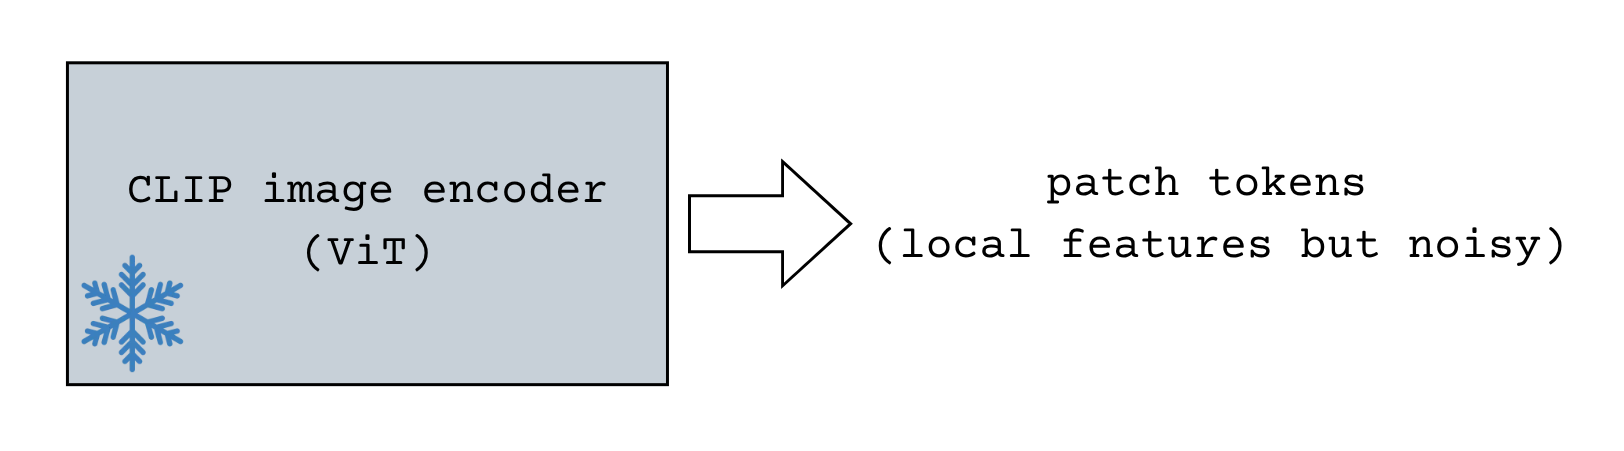
\includegraphics[width=\linewidth]{step_1.png}
        \end{column}

        % Right column
        \begin{column}{0.4\textwidth}
            \centering

            \begin{block}{\small GOAL}
                Semantically similar regions should have similar representations.
            \end{block}
            % \vspace{0.5cm}

            \uncover<2->{
                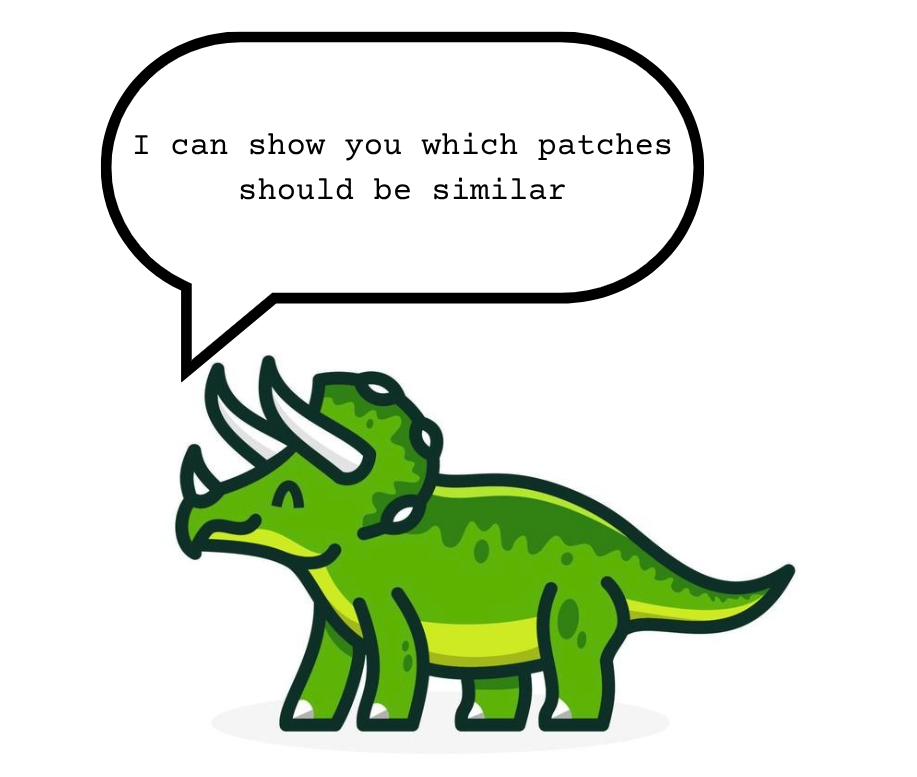
\includegraphics[width=0.8\linewidth]{step_2.png}
            }
        \end{column}
    \end{columns} 
\end{frame}

% -------------------------------------------------
\begin{frame}{Guided pooling}
    % \framesubtitle{METHOD}
    \begin{columns}[onlytextwidth]
        % Left column
        \begin{column}{0.55\textwidth}
            \centering
            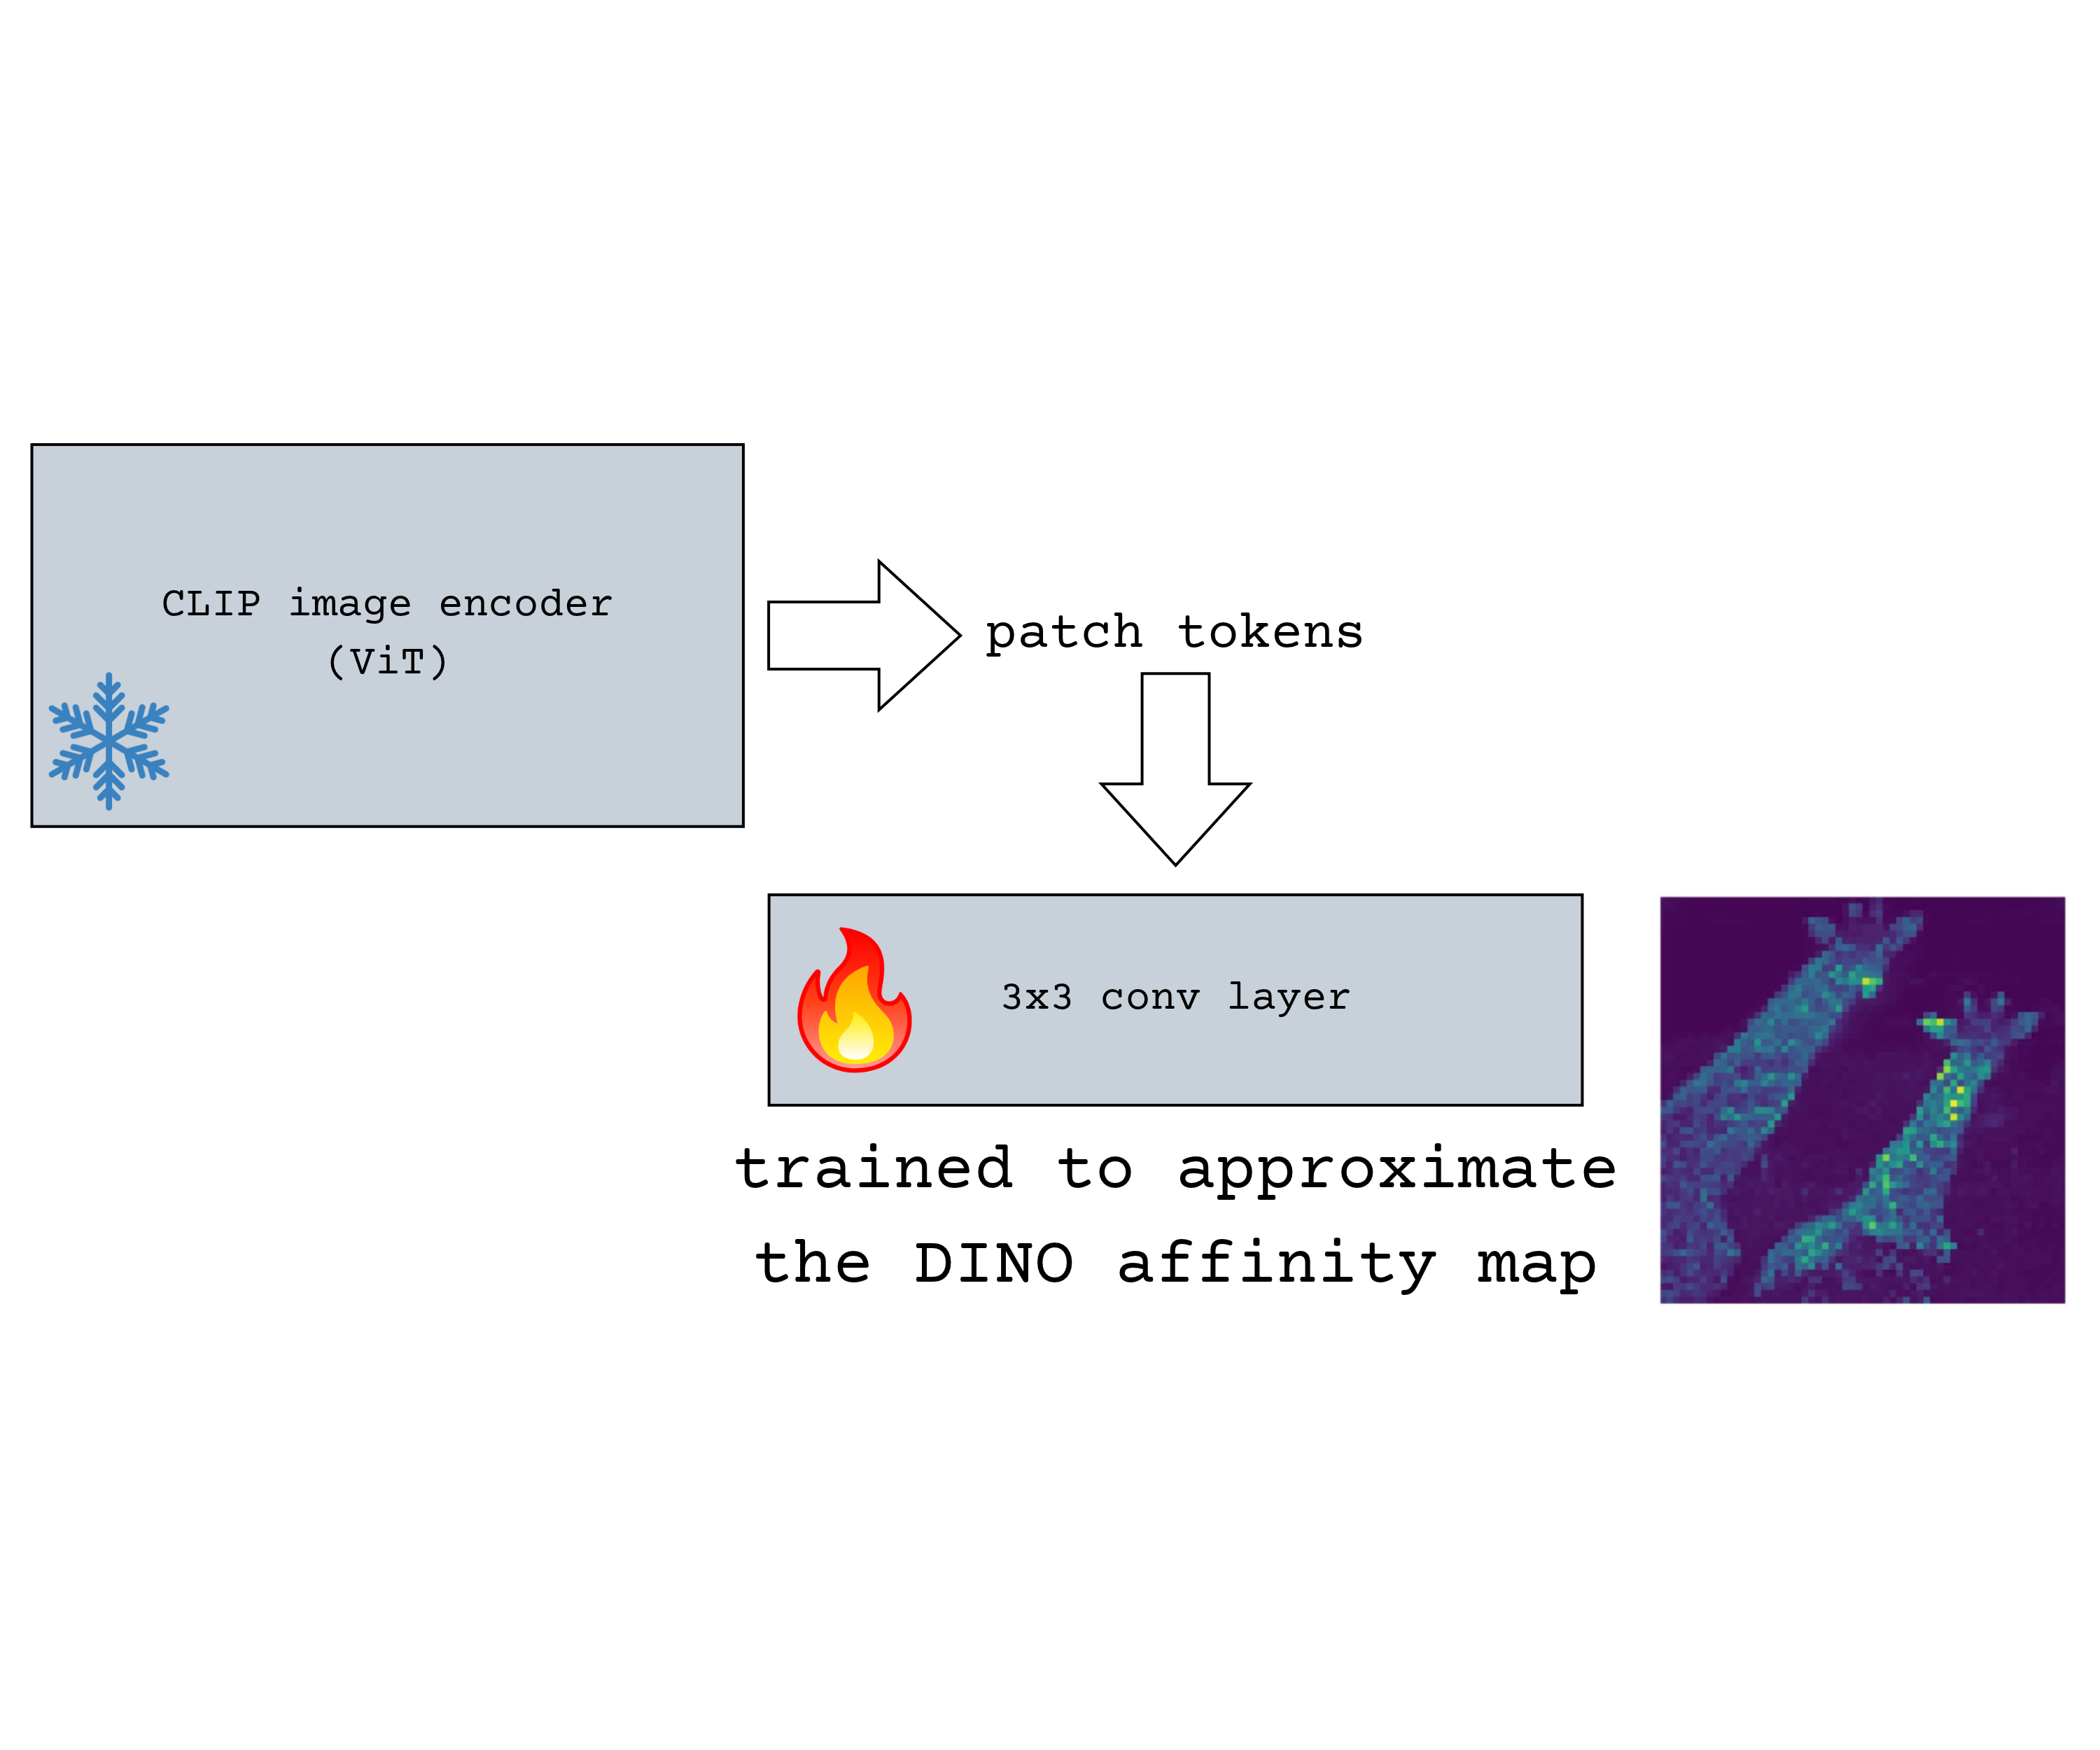
\includegraphics[width=\linewidth]{DINOiser.png}
        \end{column}

        % Right column
        \begin{column}{0.43\textwidth}
            \centering \small

            \begin{block}{\small POOLING FORMULA}
                \(F_q\): local feature of patch \(q\) \\
                \(A_{p,q}\): affinity between patches \(p\) and \(q\) \\

                \[
                    F_p^{+} =
                    \frac{\sum_{q=1}^{N} A_{p,q} F_q}
                         {\sum_{q=1}^{N} A_{p,q}}
                \]
            \end{block}

            \begin{itemize}
                \item Similar patches have a strong influence.
                \item Dissimilar patches contribute less \\ or are ignored.
            \end{itemize}
        \end{column}
    \end{columns} 
\end{frame}

% -------------------------------------------------
\begin{frame}{DINOised representations}
    % \framesubtitle{METHOD}
    \begin{figure}
        \centering
        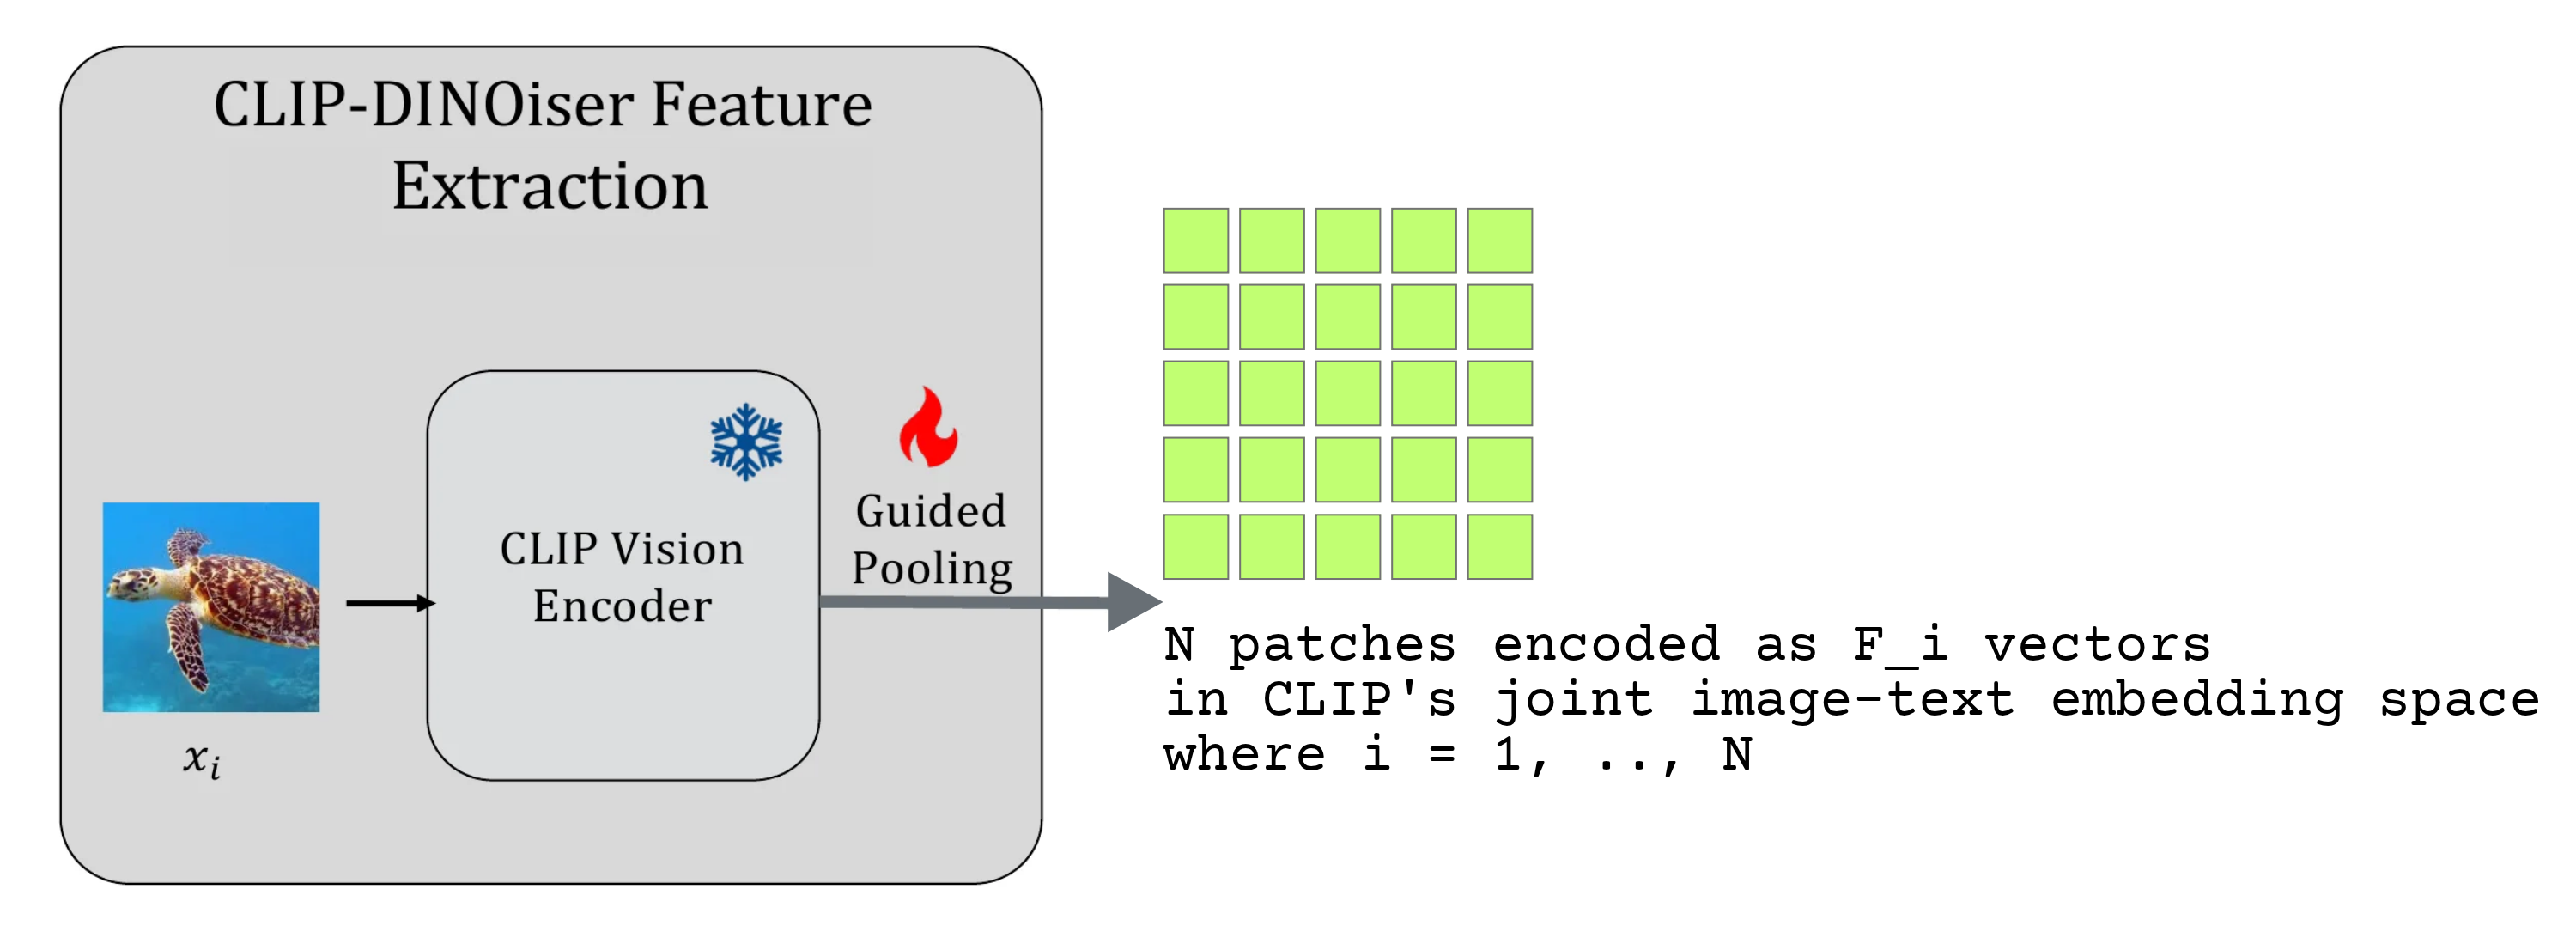
\includegraphics[width=0.75\linewidth]{DINOised_repr.png}
    \end{figure}
    
    \begin{itemize}
    \small
        \item \textbf{Spatially localized} — each representation corresponds to an image patch.
        \item \textbf{Less noisy} — Guided Pooling reduces noise in local representations.
        \item \textbf{Semantically smoother} — visually similar regions can have more consistent features.
        \item \textbf{Language-aligned} — the representations retain a connection to CLIP's image-text embedding space.
    \end{itemize}
\end{frame}

% -------------------------------------------------
\begin{frame}{Sparse Autoencoder for concept extraction}
    % \framesubtitle{METHOD}
    \begin{figure}
        \centering
        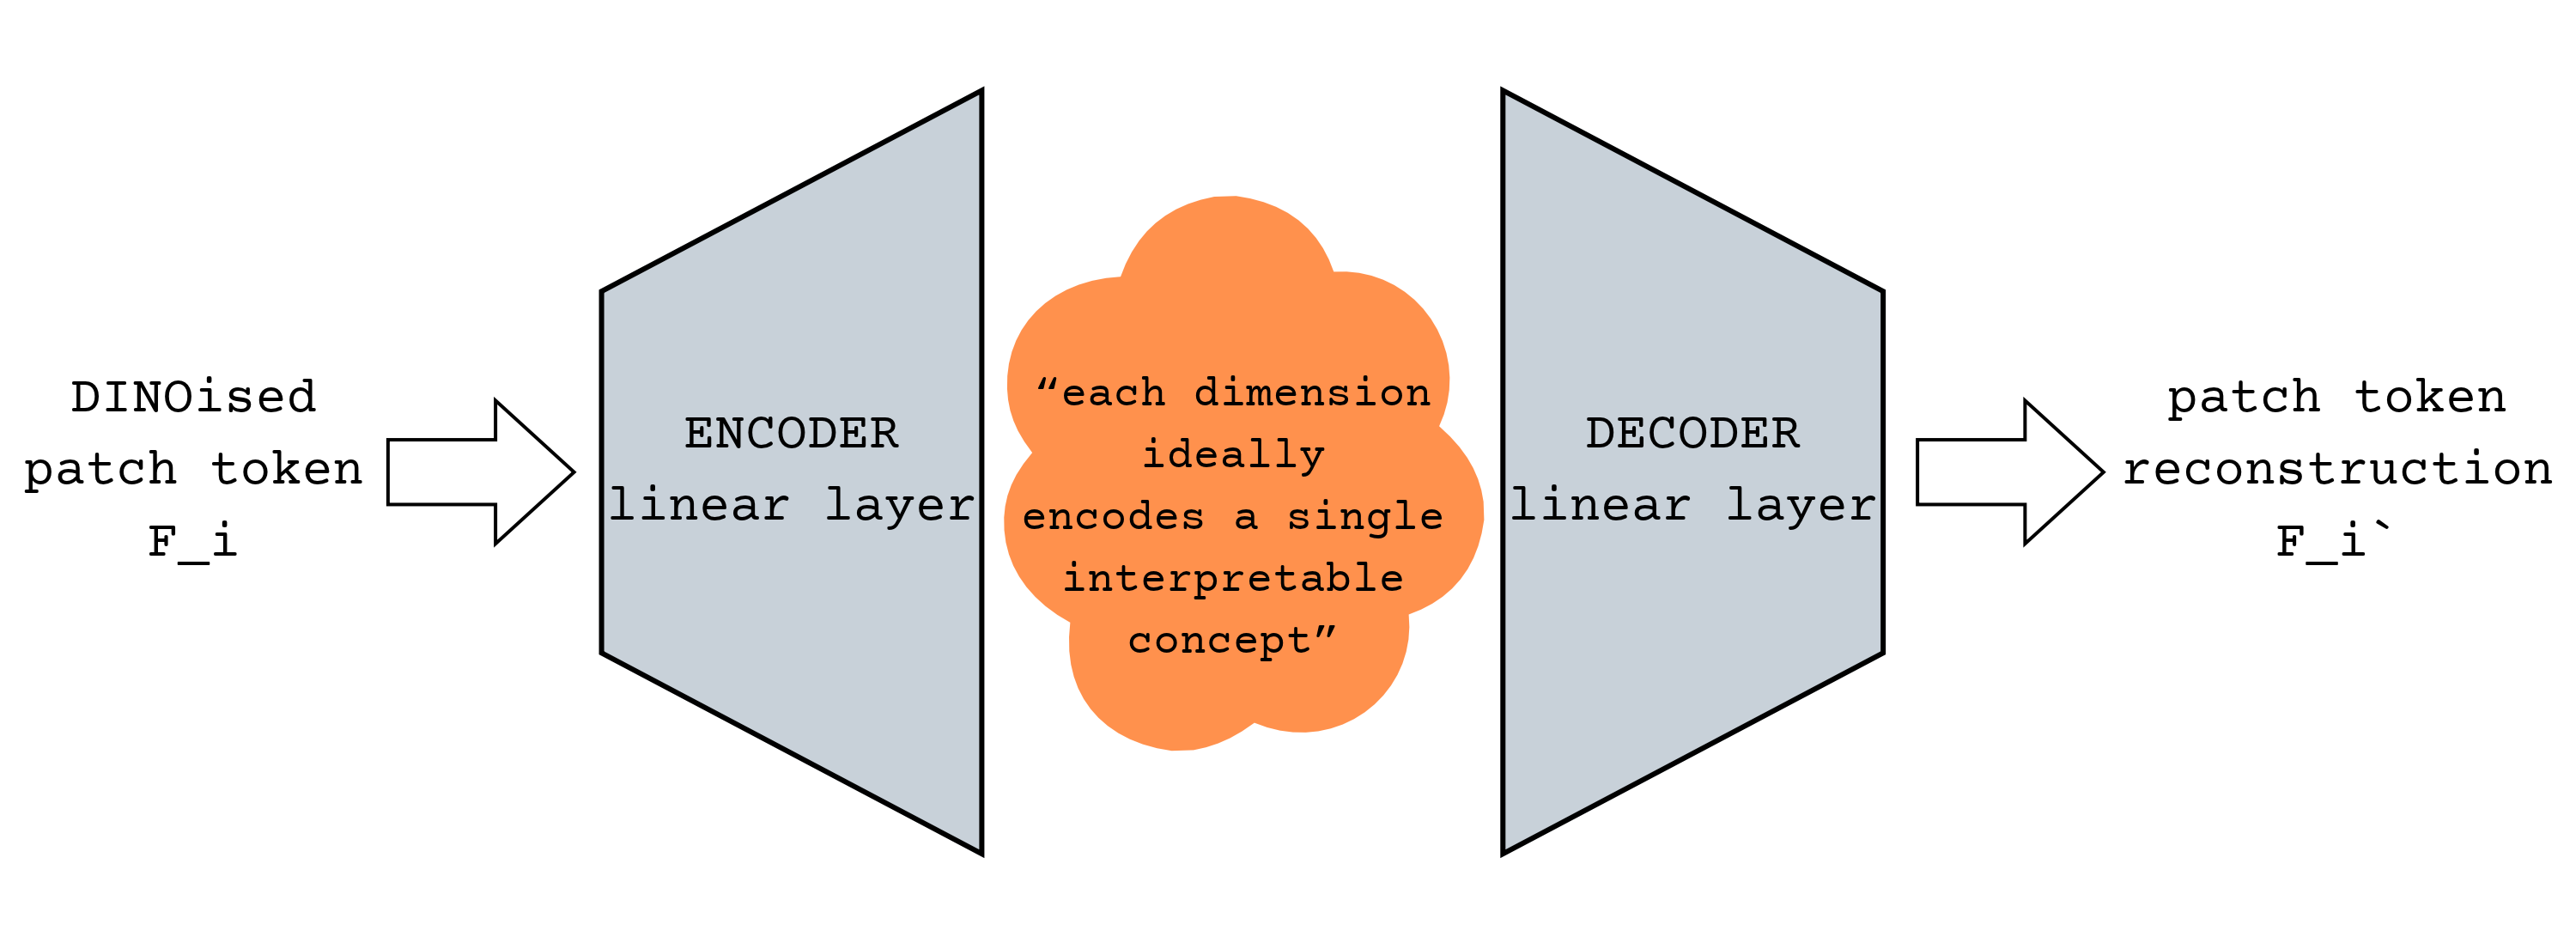
\includegraphics[width=0.8\linewidth]{SAE.png}
    \end{figure}    

    \begin{center}
        \begin{minipage}{0.4\textwidth}
            \begin{block}{\small TRAINING}
                \begin{itemize}
                    \small
                    \item reconstruction loss
                    \item sparsity regularization term
                \end{itemize}
            \end{block}
        \end{minipage}
    \end{center}
\end{frame}

% -------------------------------------------------
\begin{frame}{BatchTopK: sparsity regularization}
    % \framesubtitle{METHOD}
    \begin{columns}[onlytextwidth]
        % Left column
        \begin{column}{0.6\textwidth}
            \centering
            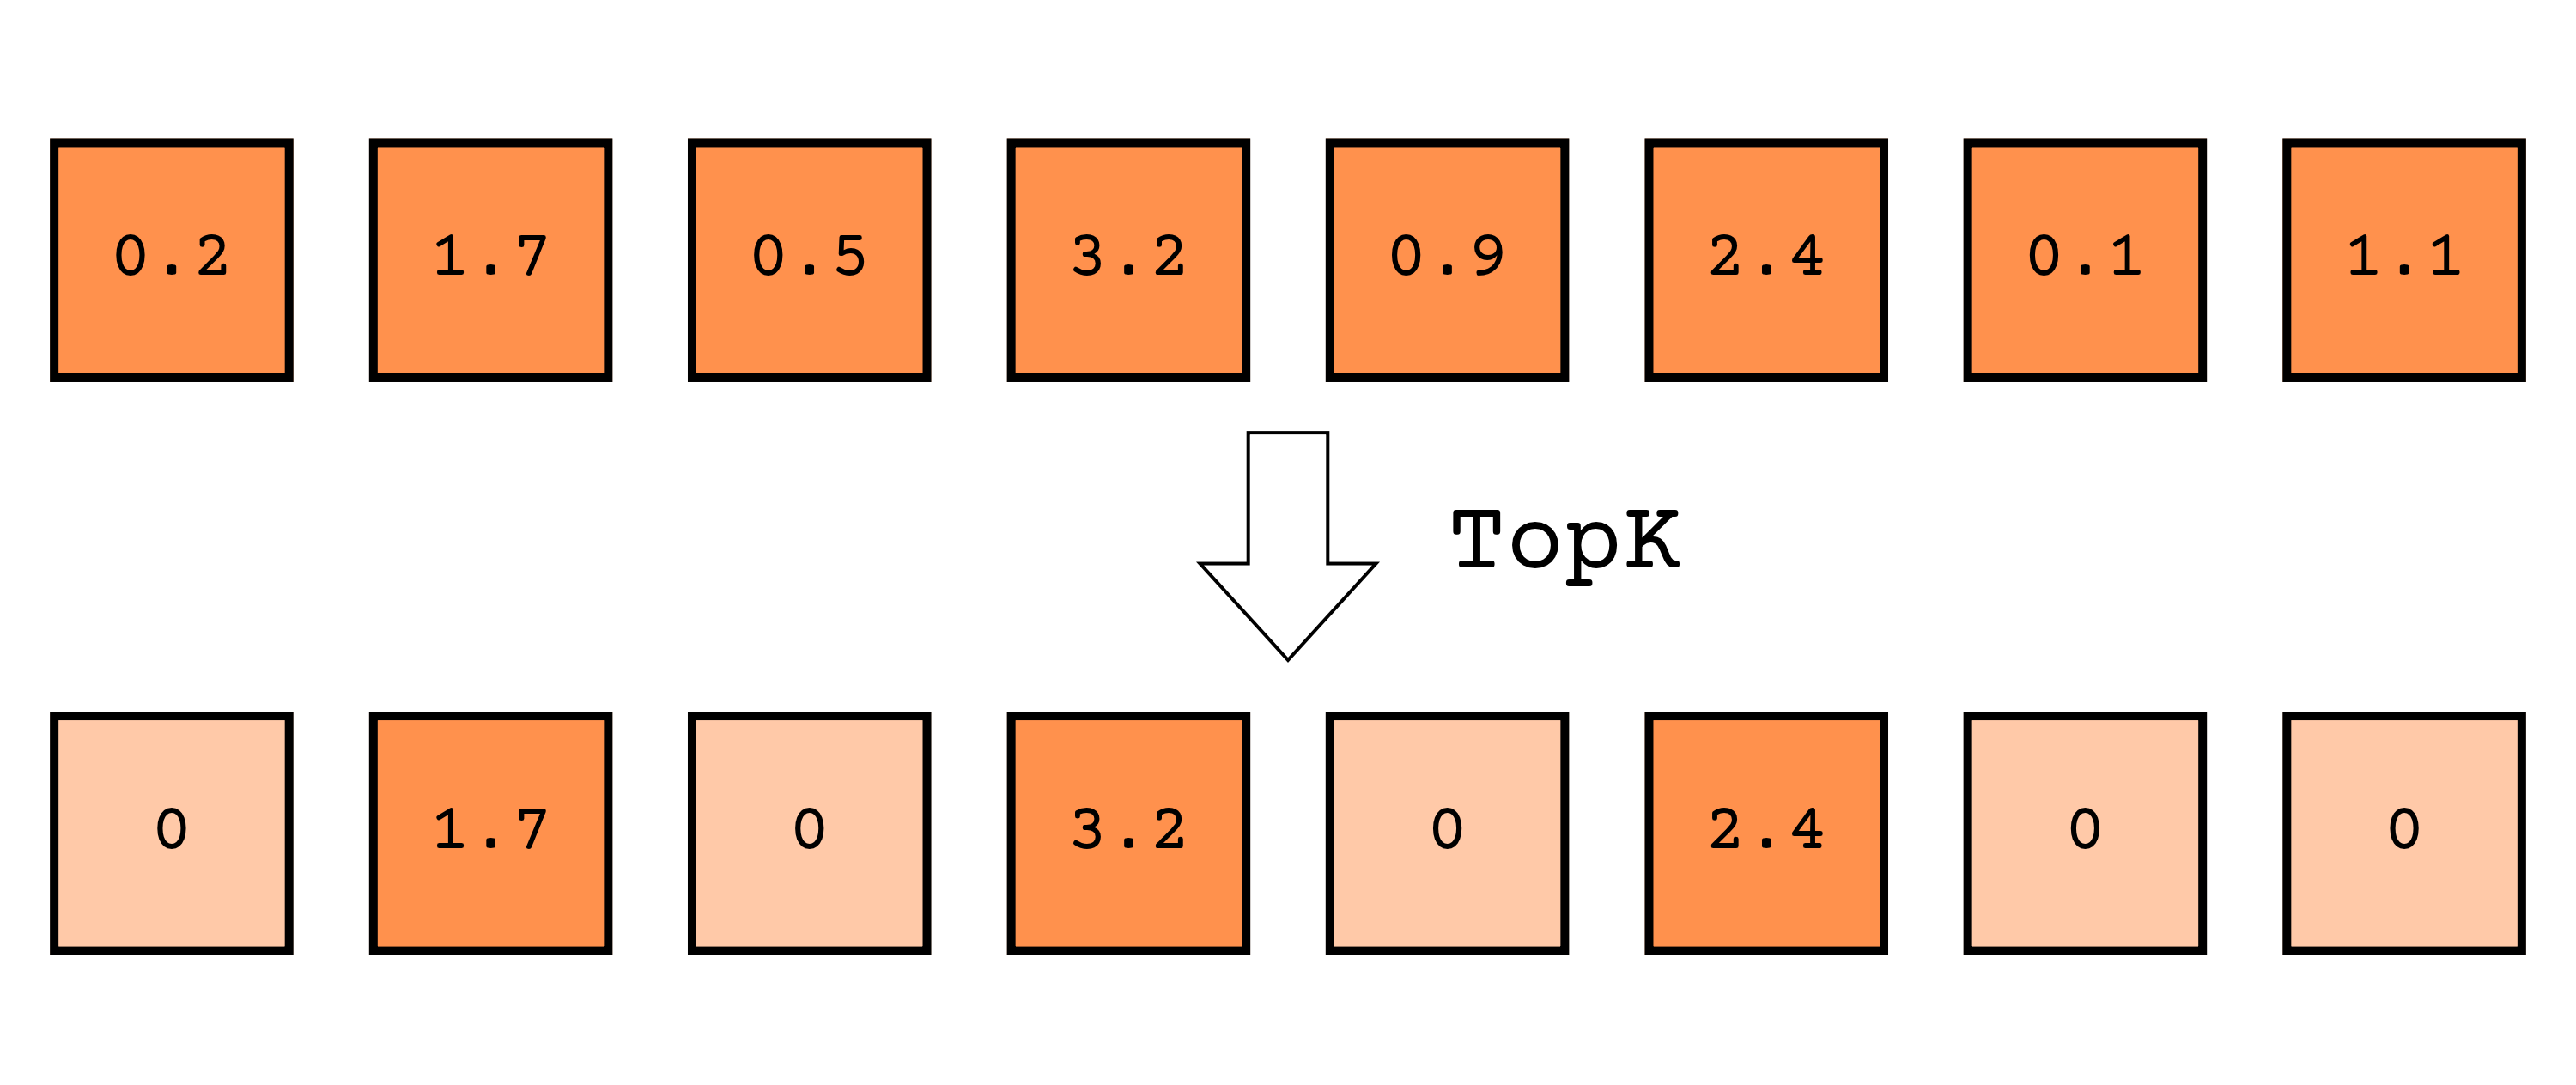
\includegraphics[width=0.9\linewidth]{topK.png}
            \centering
            \\ SAE decoder reconstructs the input using \\ only the retained activations.
        \end{column}

        % Right column
        \begin{column}{0.4\textwidth}
            \uncover<2->{
                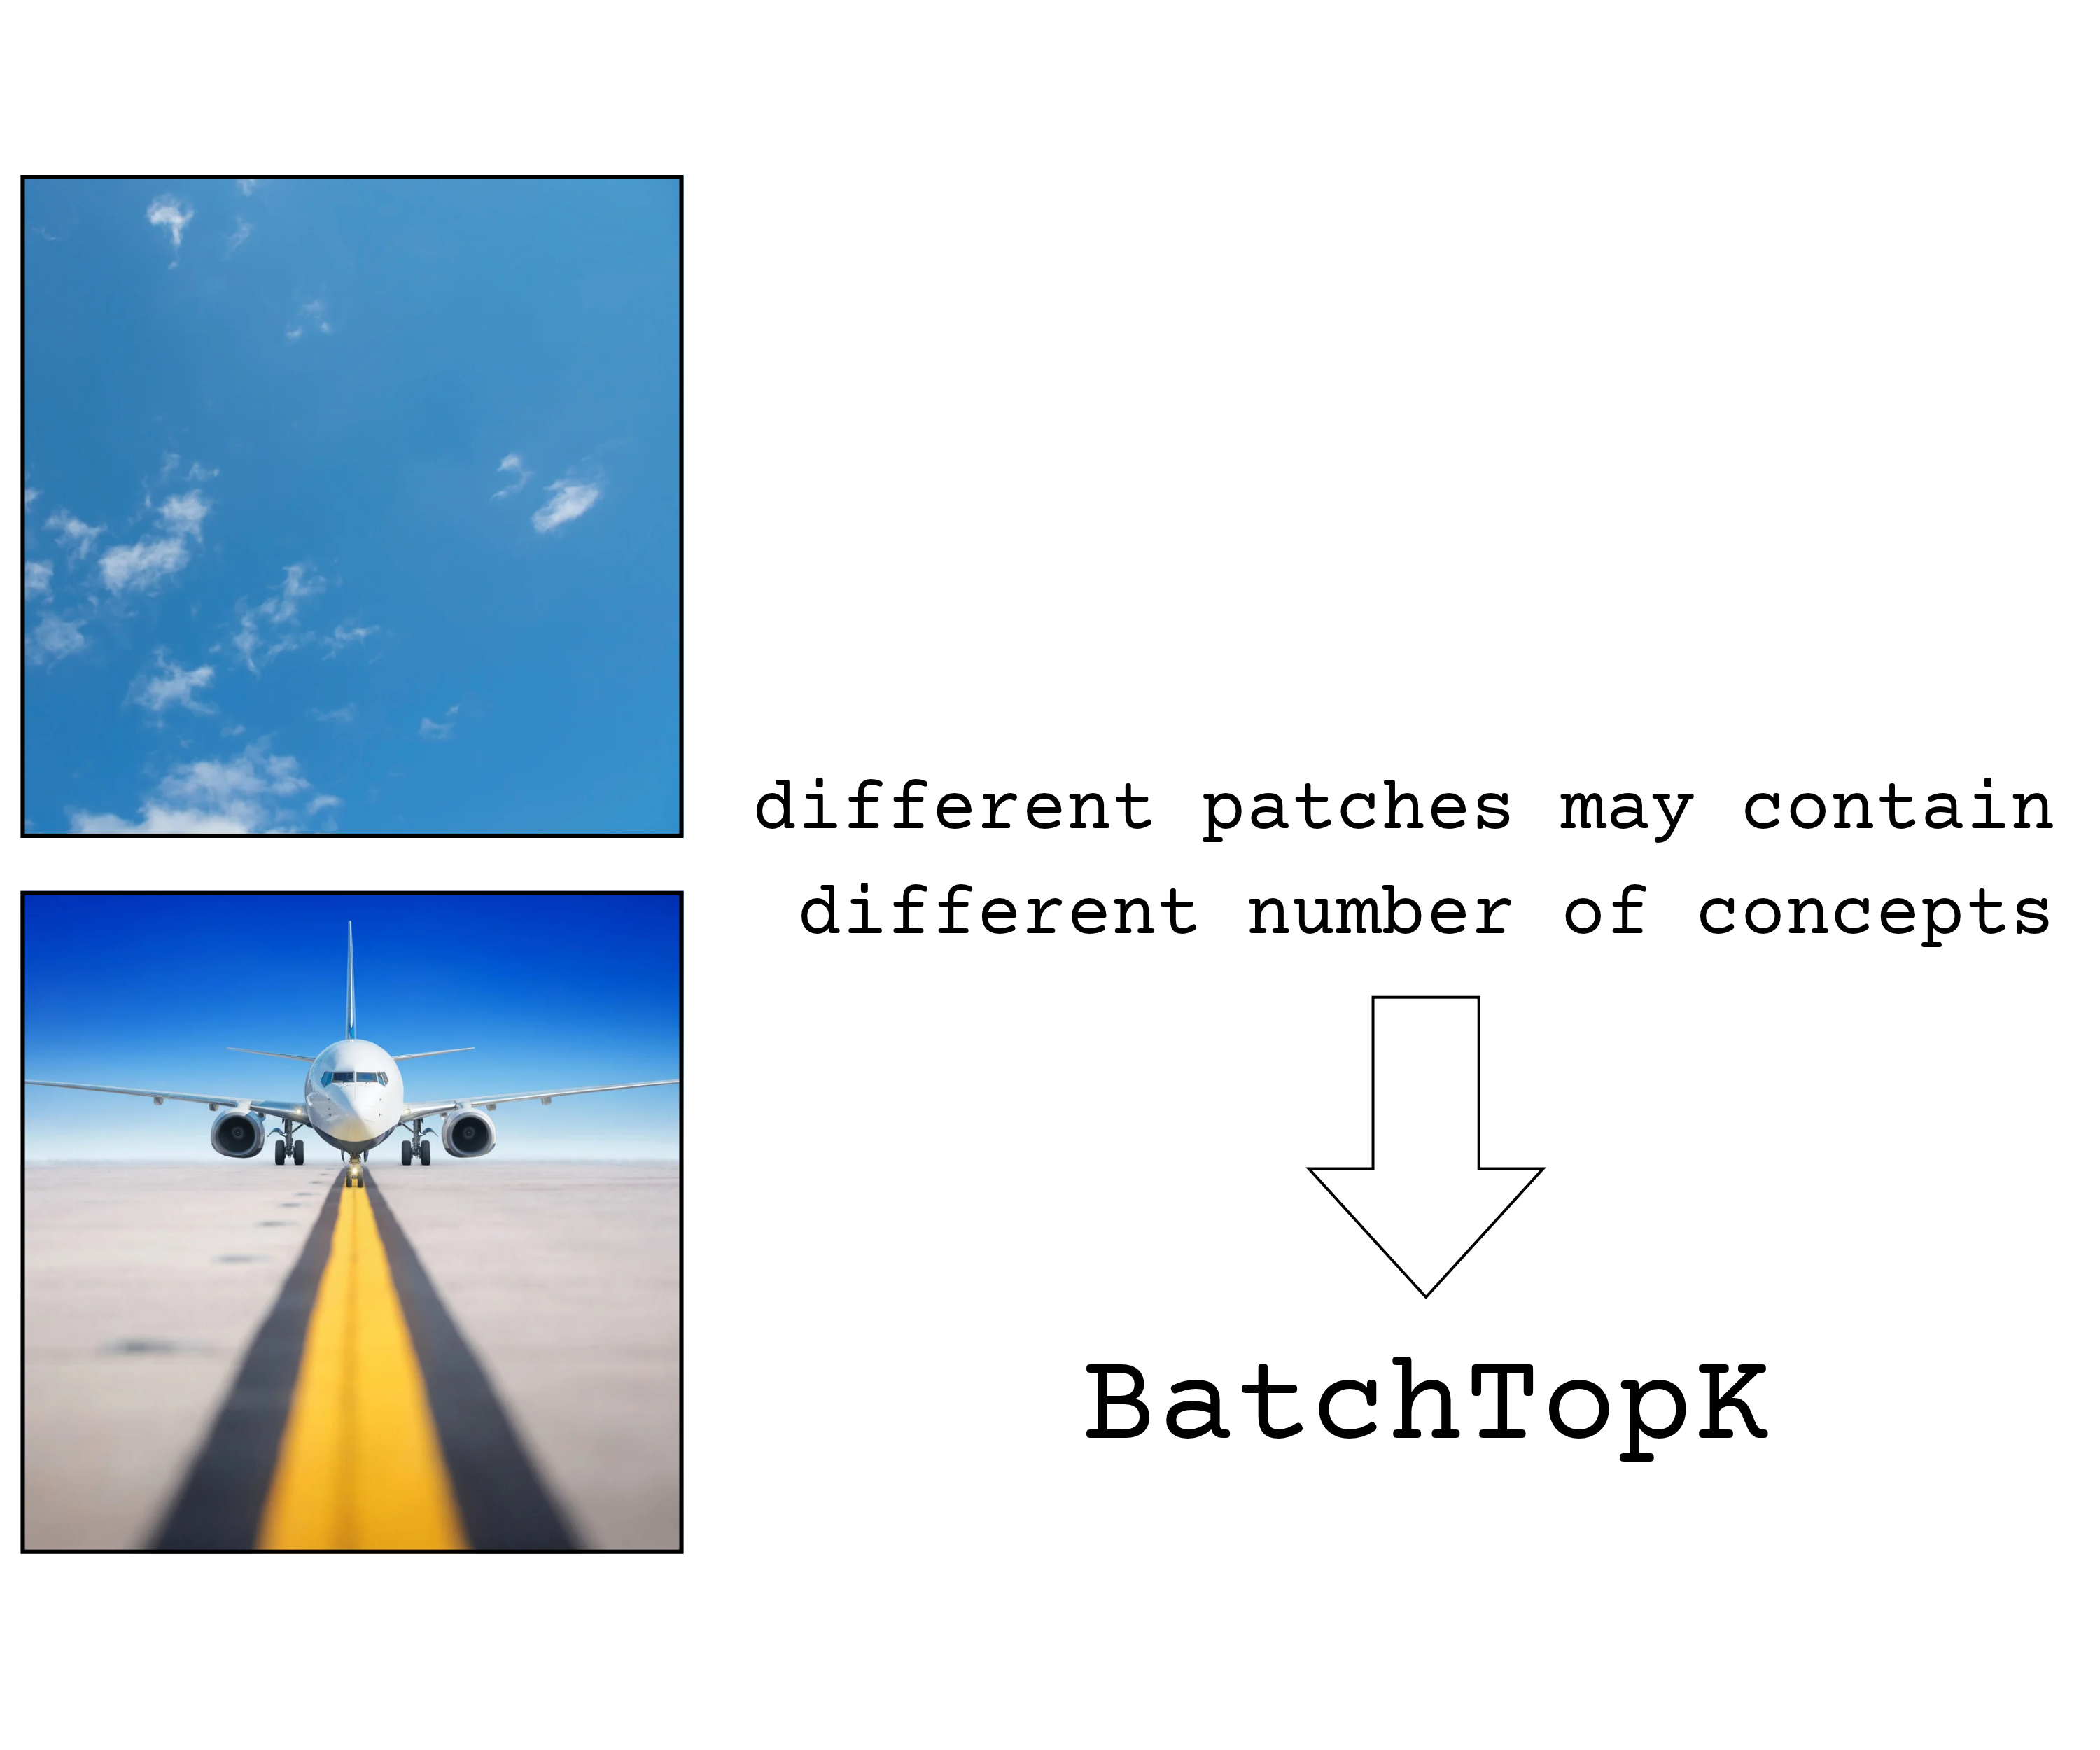
\includegraphics[width=0.95\linewidth]{batchTopK.png}
            }
        \end{column}
    \end{columns} 
\end{frame}

% -------------------------------------------------
\begin{frame}{Matryoshka objective}
    % \framesubtitle{METHOD}
    \begin{columns}[onlytextwidth]
        % Left column
        \begin{column}{0.6\textwidth}
            \centering
            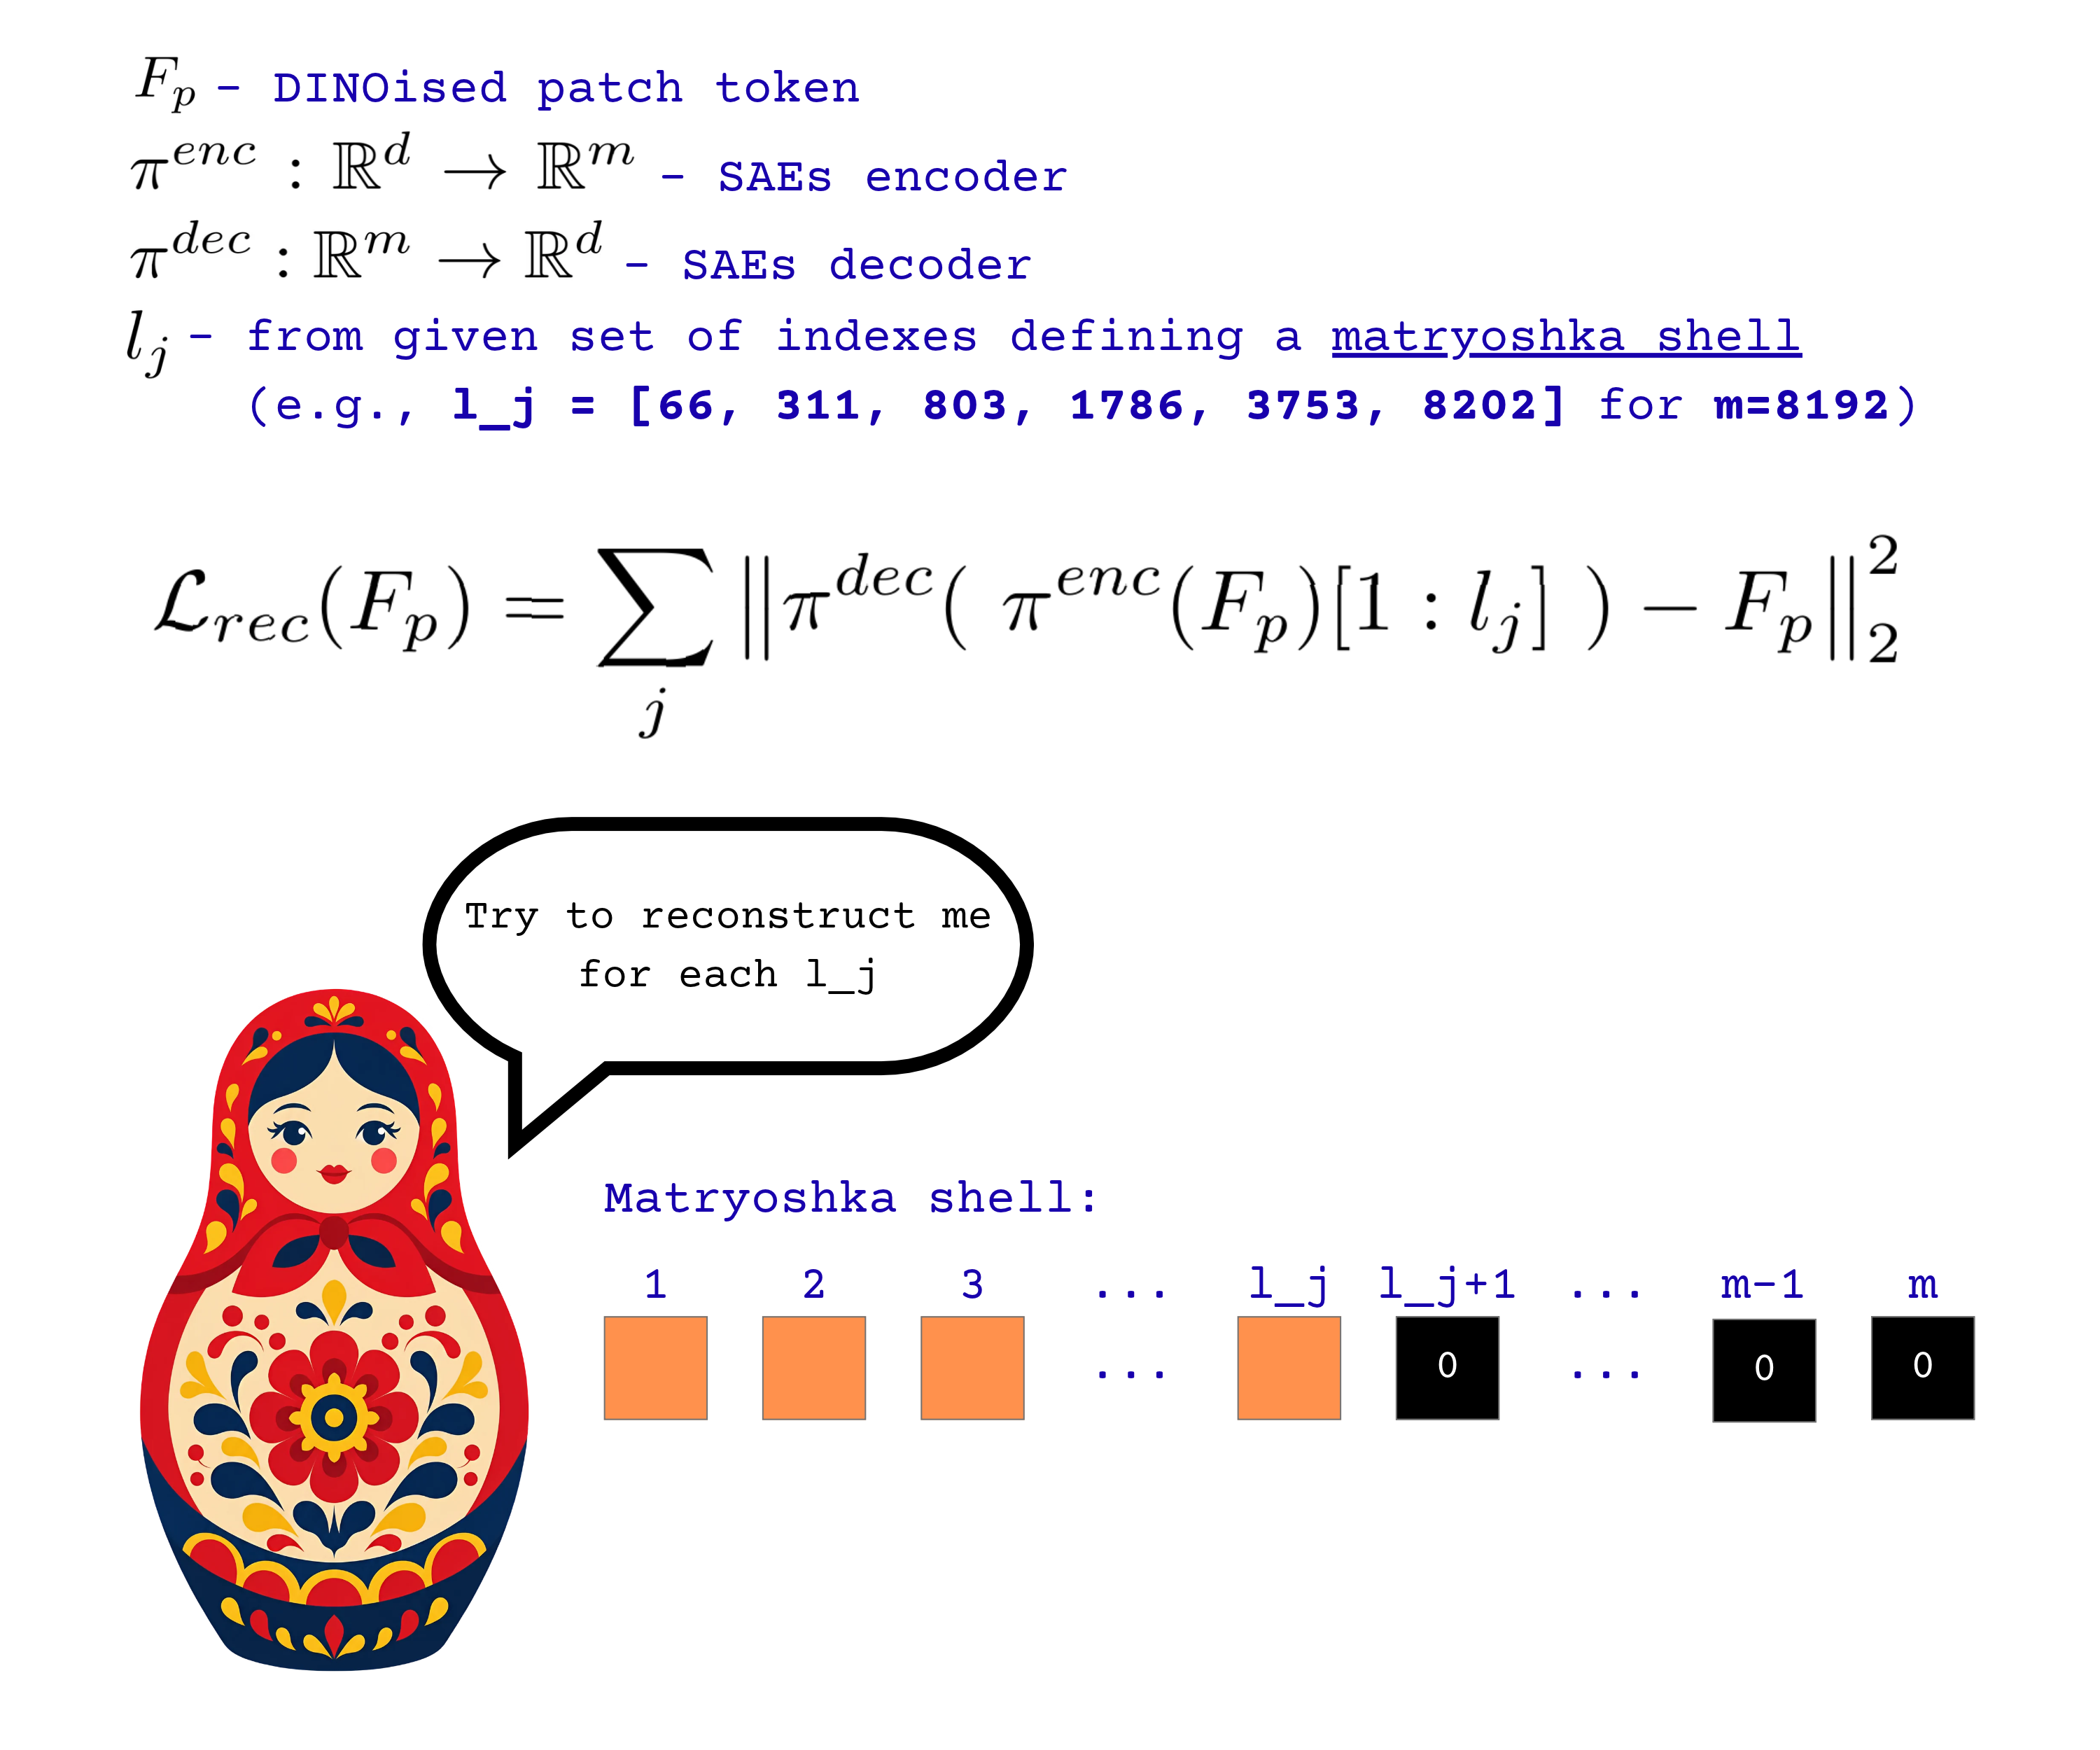
\includegraphics[width=0.9\linewidth]{matryoshka.png}
        \end{column}

        % Right column
        \begin{column}{0.4\textwidth}
                \begin{itemize}
                \small
                \uncover<2->{
                    \item Smaller parts should preserve useful information.
                    \item \textit{First neurons learn coarse, \\ high-level information.}
                }
                \uncover<3->{
                    \item Larger parts can capture more information and finer distinctions.
                    \item \textit{Higher-index neurons learn \\ the residual fine-grained information.}
                }
                \end{itemize}
        \end{column}
    \end{columns} 
\end{frame}

% -------------------------------------------------
\begin{frame}{From learned representations to named concepts}
    % \framesubtitle{METHOD}
    \begin{columns}[onlytextwidth]
        % Left column
        \begin{column}{0.35\textwidth}
        \scriptsize
        \textbf{Learned representations:} \\ localized concepts at diverse granularities. \\
        \vspace{0.2cm}
        \textbf{Remaining challenge:} \\ the dimensions in concept space \\ do not have human-readable names. \\
        \vspace{0.2cm}
        \textbf{Next step:} \\ identify concepts and assign labels.
        \end{column}
        
        % Right column
        \begin{column}{0.65\textwidth}
            \centering
            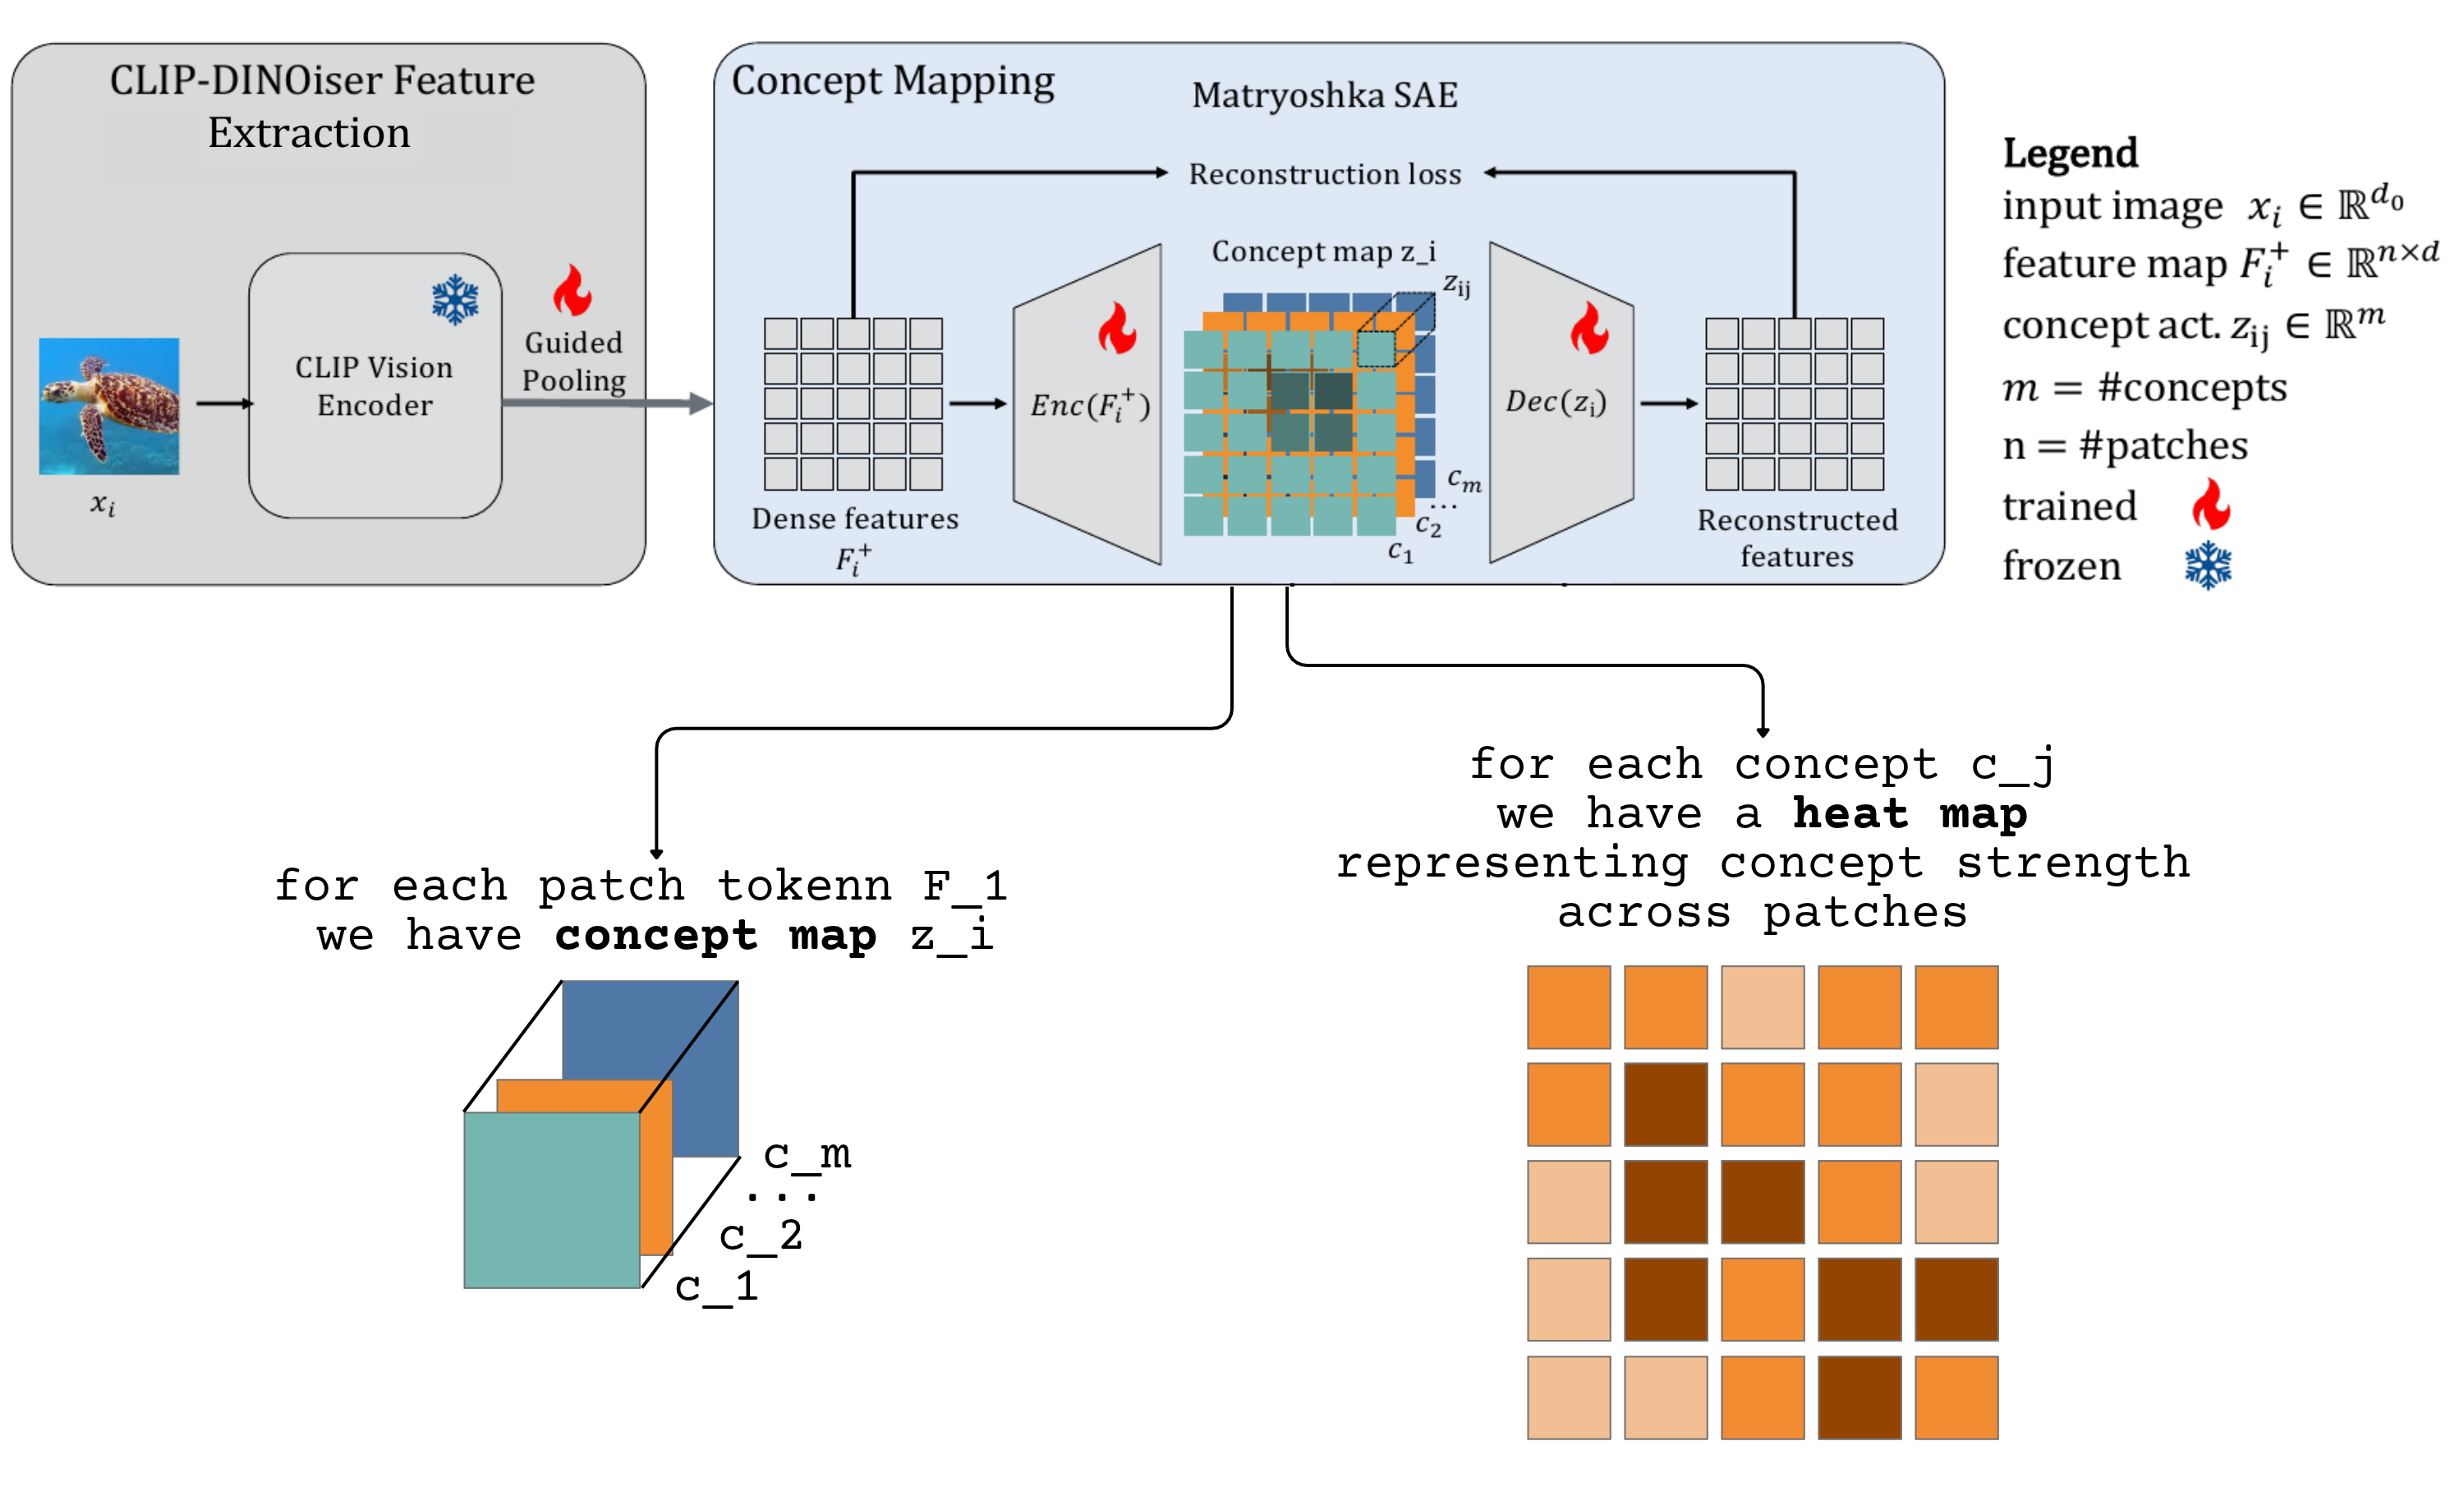
\includegraphics[width=\linewidth]{step_3.png}
        \end{column}
    \end{columns} 
\end{frame}

% -------------------------------------------------
\begin{frame}{Discovering inter-concept relationships}
    % \framesubtitle{METHOD}
    \begin{figure}
        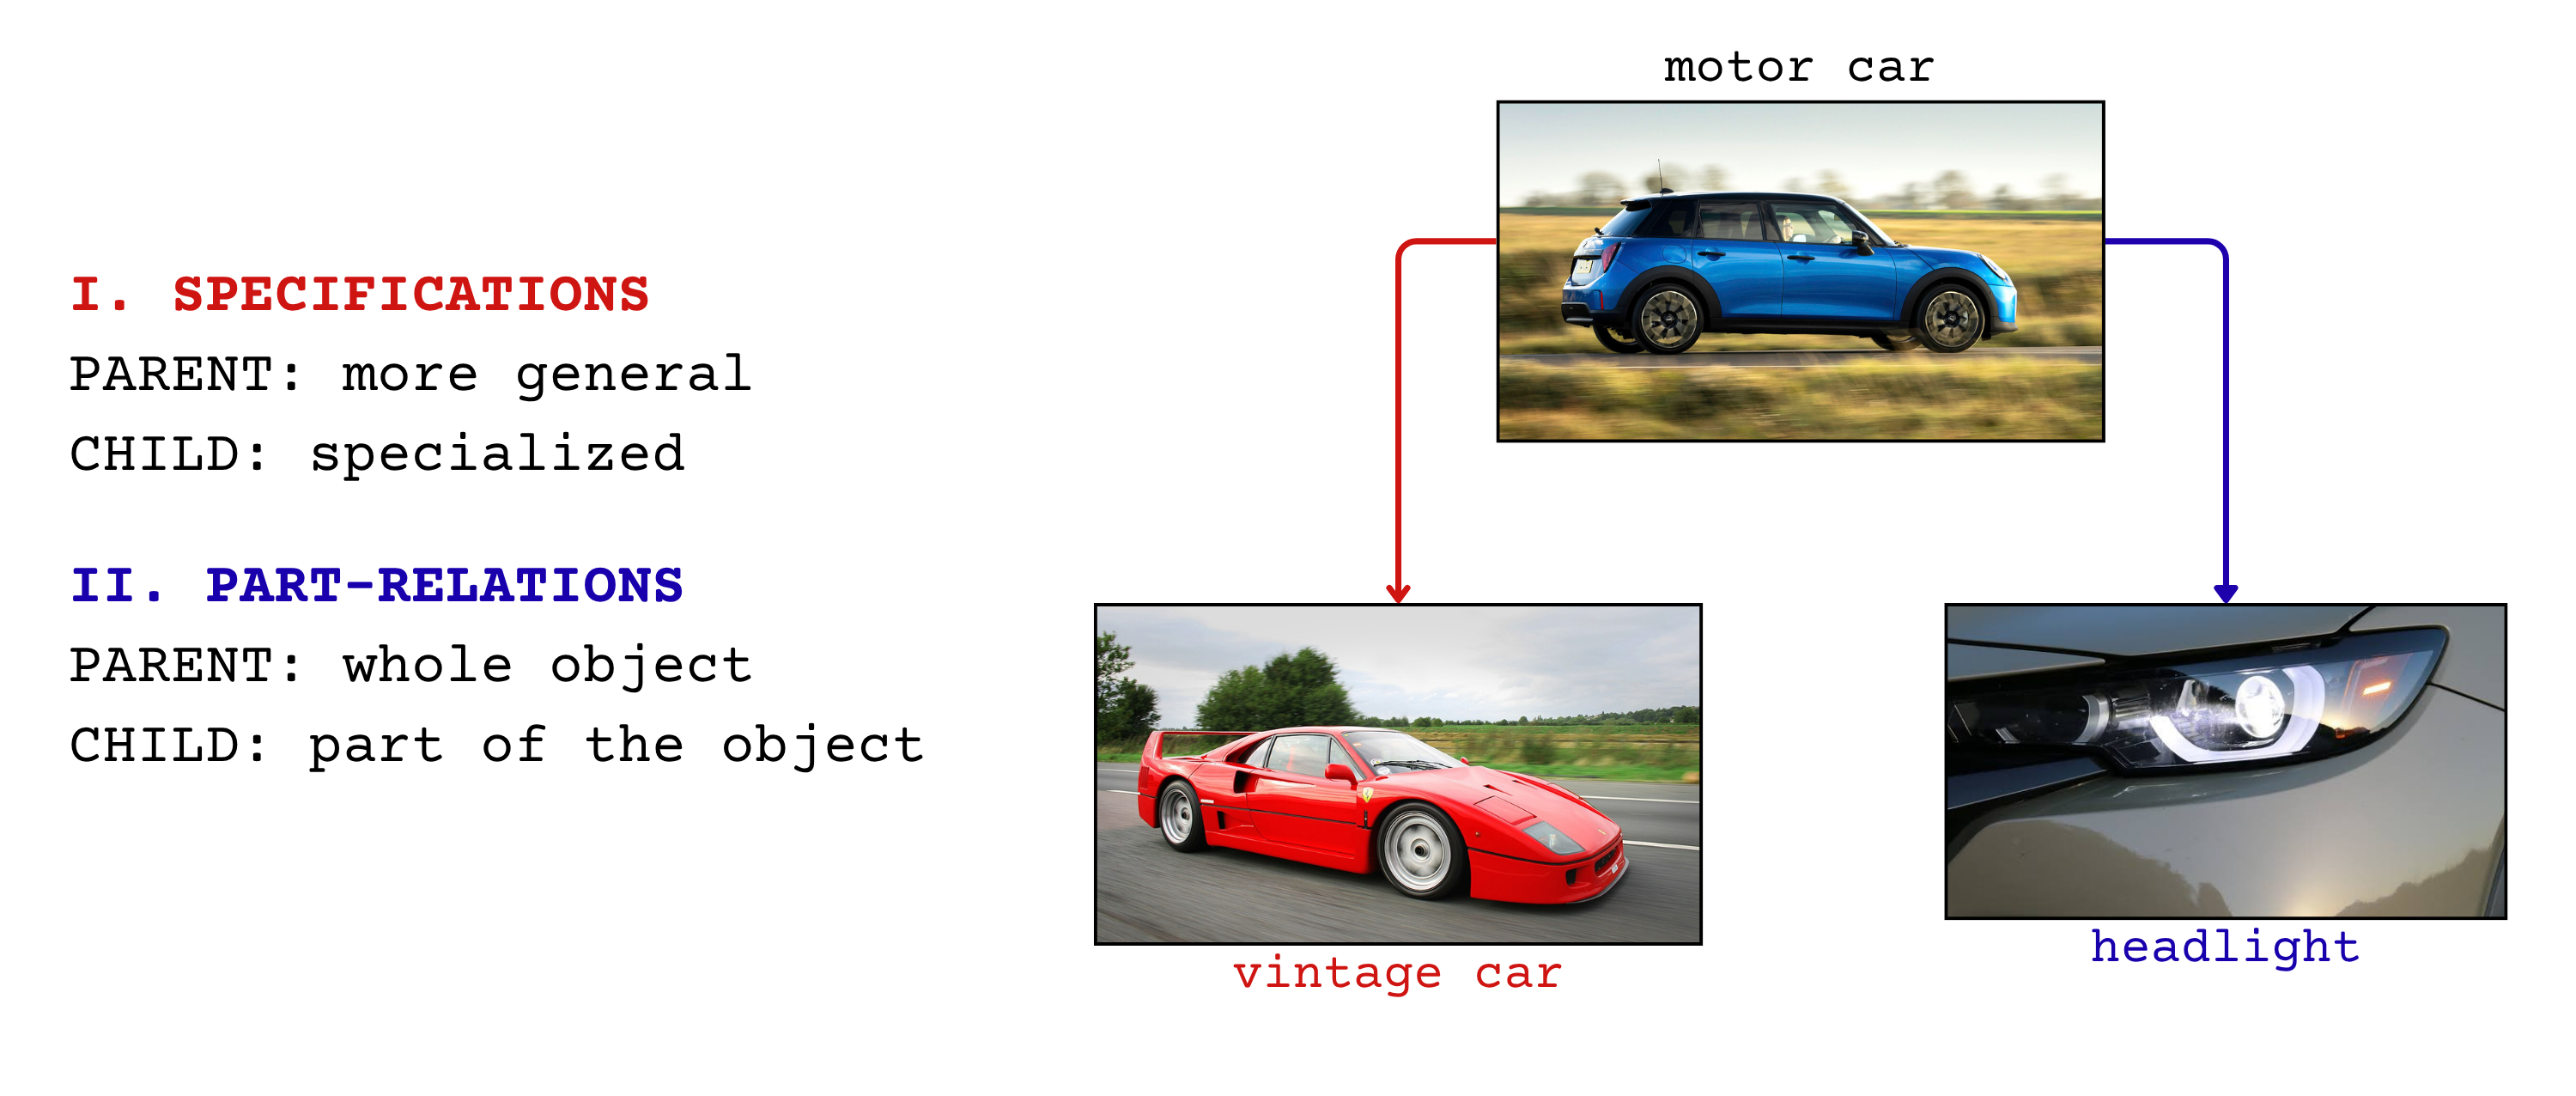
\includegraphics[width=0.75\linewidth]{relations.png}
    \end{figure}

    \vspace{-1cm}
    \uncover<2->{
    \begin{center}
        \begin{minipage}{0.75\textwidth}
            \begin{block}{\small Hierarchy Criterion:}
            \small
            CHILD concept is active $\implies$ PARENT concept should also be active
        \end{block}
        \end{minipage}
    \end{center}
    }
\end{frame}

% -------------------------------------------------
\begin{frame}{Measuring concept co-occurrence}
    % \framesubtitle{METHOD}
        \begin{columns}[T, onlytextwidth]
        % Left column
        \begin{column}{0.48\textwidth}
        \begin{block}{\footnotesize Concept co-occurrence matrix: $C \in [0, 1]^{m \times m}$}
            \footnotesize
            where $C_{ij}$ is \textit{conditional probability} \\ of concept $c_i$ (potential PARENT) being active given the concept $c_j$ (potential CHILD) is active         
        \end{block}
        
        \vspace{-0.35cm}
        \begin{figure}
            \centering
            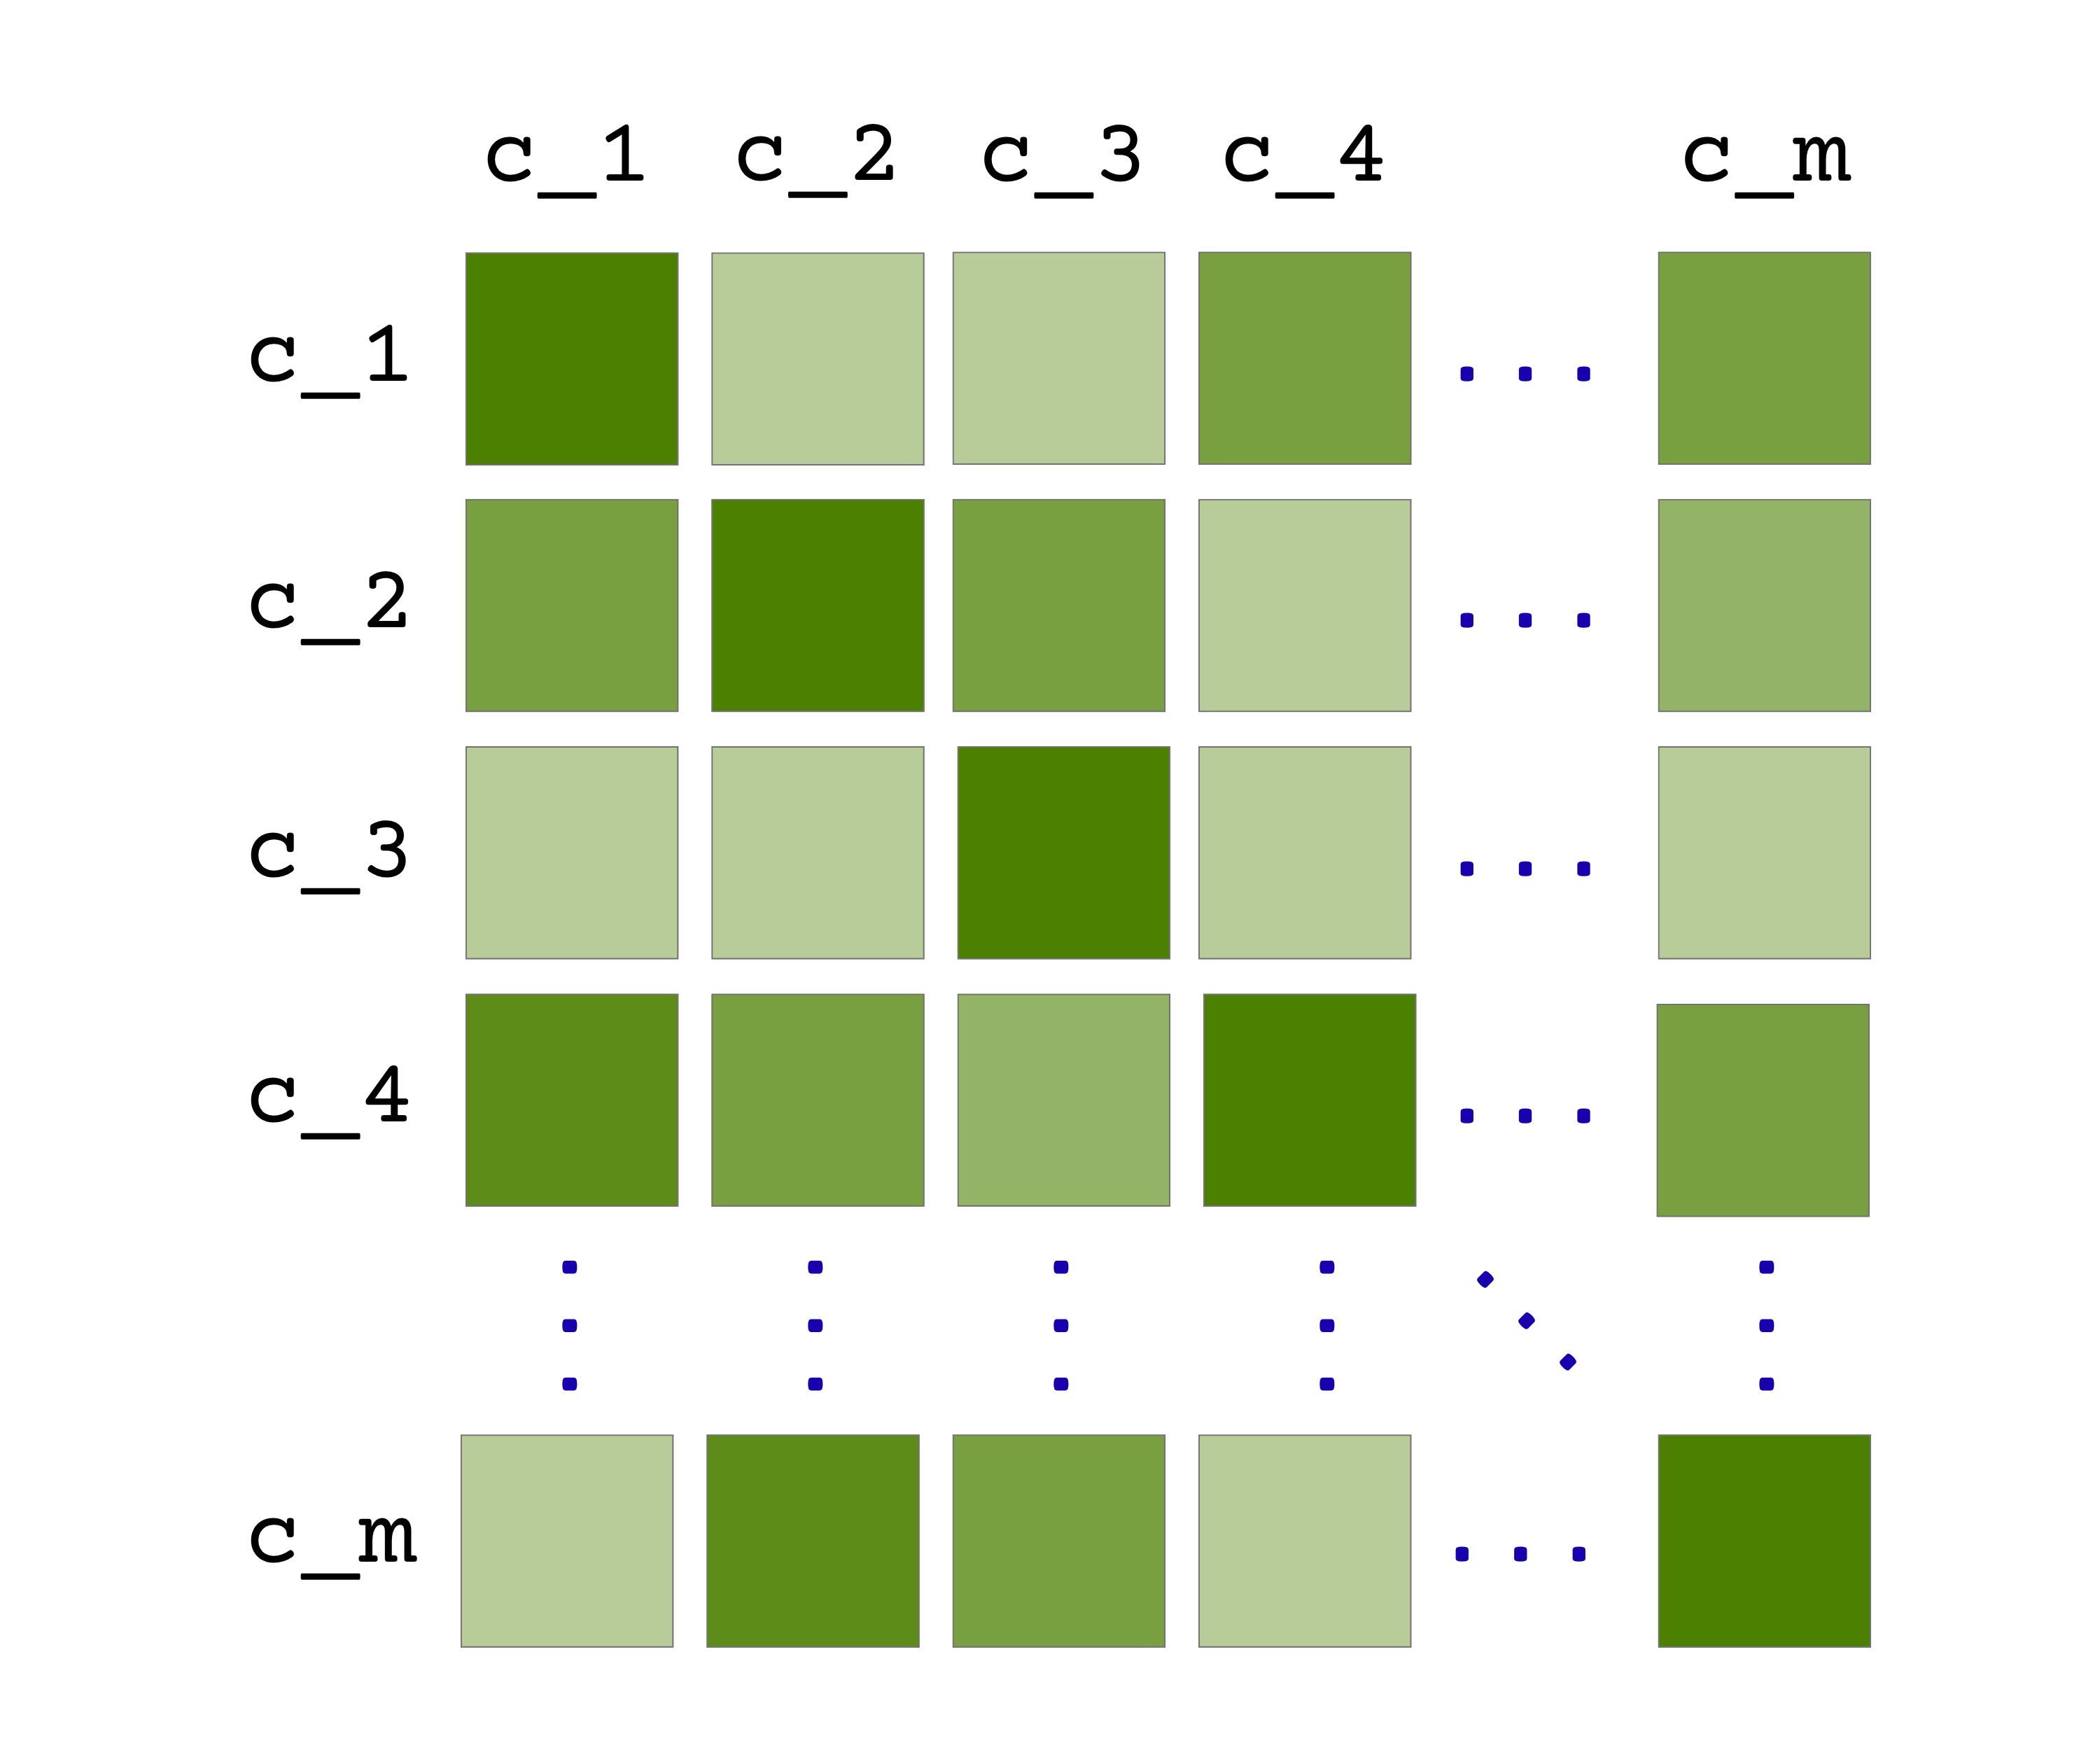
\includegraphics[width=0.35\linewidth]{matrix.png}
        \end{figure}
        
        \vspace{-0.5cm}
        \uncover<7->{
            \begin{block}{\footnotesize Do we have PARENT $c_i$ $\xrightarrow{}$ CHILD $c_j$ relationship?}
            \footnotesize
            for a chosen threshold $\tau$ (e.g., $\tau=0.75$) \\
            \begin{itemize}
                \item YES - if $C_{ij} \ge \tau$
                \item NO  - otherwise
            \end{itemize}
            \end{block}
        }
        \end{column}
        
        % Right column
        \begin{column}{0.48\textwidth}
        \begin{block}{\footnotesize Calculating $C_{ij}$:}
            \begin{itemize}[<+->]
            \footnotesize
                \item $A_{jp}$ - activation value of concept $c_j$ for patch $p$
                \item $p:j \in B(p)$ - select all patches $p$ for which the CHILD concept $c_j$ is active
                \item $\sum_{p:j \in B(p)}A_{jp}$ - sum the activations of the~CHILD concept $c_j$ across the selected patches
                \item $p:j,i \in B(p)$ - select all patches $p$ for which both the PARENT concept $c_i$ and the CHILD concept $c_j$ are active
                \item $\sum_{p:j,i \in B(p)}A_{jp}$ - sum the activations of the CHILD concept $c_j$ across the selected patches
                \item $C_{ij} = \frac{\sum_{p:j,i \in B(p)}A_{jp}}{\sum_{p:j \in B(p)}A_{jp}}$
            \end{itemize}       
        \end{block}
        \end{column}
    \end{columns} 
\end{frame}

% -------------------------------------------------
\begin{frame}{From concepts to language}
    % \framesubtitle{METHOD}
    \begin{columns}[onlytextwidth]
        % Left column
        \begin{column}{0.48\textwidth}
            \begin{block}{\small Concept dictionary vector $\pi^{dec}_i$}
                \scriptsize
                $\pi^{dec}:\mathbb{R}^m\to\mathbb{R}^d$ - SAE decoder affine map \\
                $W^{dec}\in\mathbb{R}^{d\times m}$ - decoder weight matrix \\
                $b^{dec}$ - decoder bias vector \\
                $e_i\in\mathbb{R}^m$ - one-hot vector corresponding to concept $c_i$ \\
                
                \[
                \begin{aligned}
                \pi^{dec}(e_i)
                &= W^{dec}e_i+b^{dec}\\
                &= \boldsymbol{W^{dec}_{:,i}}+b^{dec}\\
                &= \boldsymbol{\pi_i^{dec}}+b^{dec}
                \end{aligned}
                \]

                \vspace{0.2cm}
                The concept dictionary vector for concept \(c_i\)
                is the \textbf{\(i\)-th column} of the decoder weight matrix:
                \[
                \pi_i^{dec} = W^{dec}_{:,i}
                \]
                \vspace{0.01cm}
            \end{block}
        \end{column}

        % Right column
        \begin{column}{0.48\textwidth}
            \uncover<2->{
            \begin{block}{\small Standard Approach}
                \scriptsize
                \vspace{0.2cm}
                \[
                l_i = \argmax\nolimits_{v \in \mathcal{V}}
                \cos\left(\pi_i^{dec}, \mathcal{T}(v)\right)
                \]
                \begin{itemize}
                    \item $\mathcal{V}$ - pre-defined vocabulary of candidate labels
                    \item $\mathcal{T}(v) \in \mathbb{R}^d$ - CLIP text embedding of $v \in \mathcal{V}$
                    \item $l_i$ - label assigned to concept $c_i$
                \end{itemize}
                \vspace{0.2cm}
            \end{block}
            }
        \end{column}
    \end{columns}
\end{frame}

% -------------------------------------------------
\begin{frame}{Taking parents into account can help}
    % \framesubtitle{METHOD}
    \begin{figure}
        \centering
        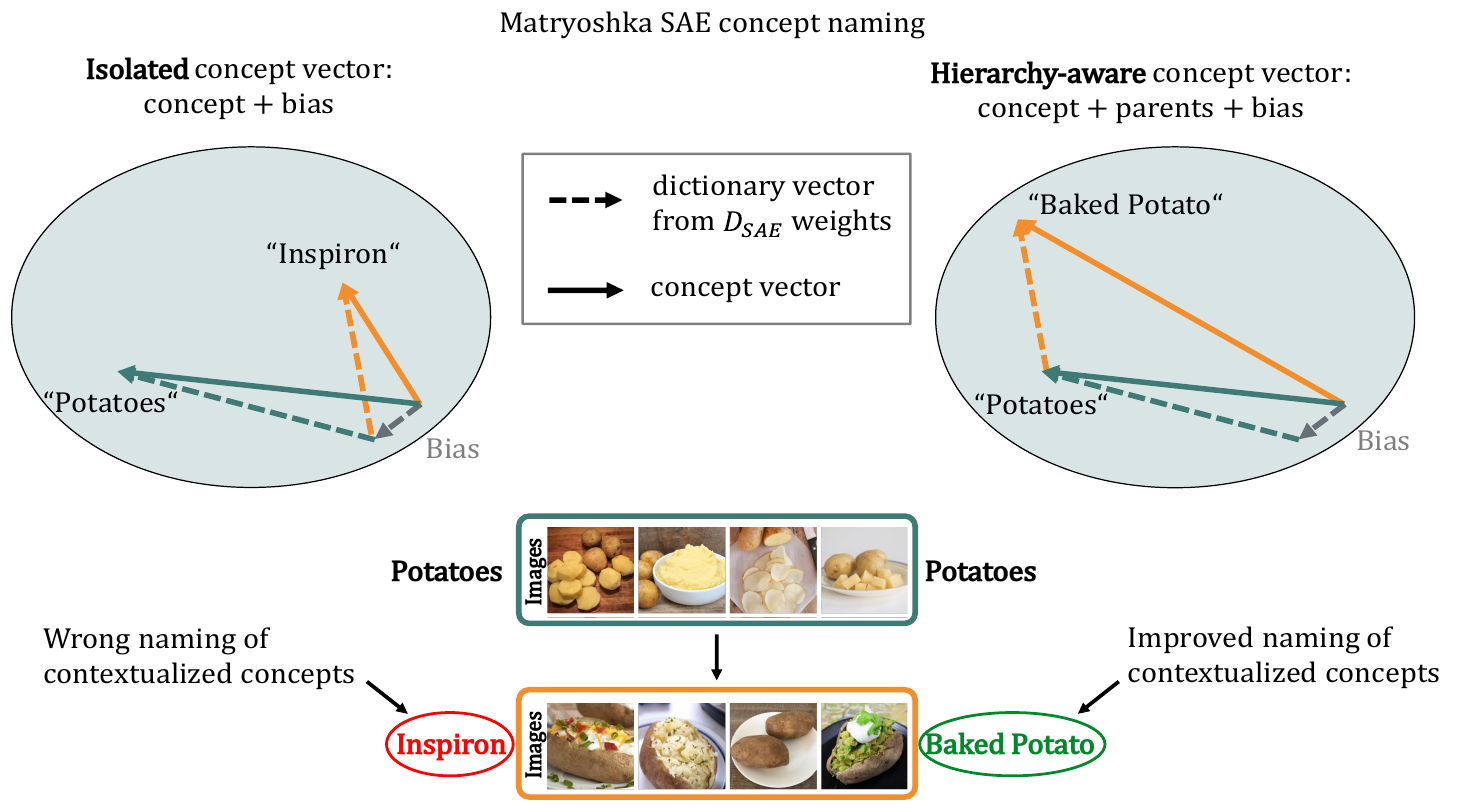
\includegraphics[width=0.75\linewidth]{namin_problem.png}
    \end{figure}
\end{frame}

% -------------------------------------------------
\begin{frame}{Hierarchy-aware concept naming}
    % \framesubtitle{METHOD}
    \vspace{-0.35cm}
    \begin{center}
    \begin{minipage}{0.8\textwidth}
    \begin{block}{}
    {
    \scriptsize
    \[
    l_j =
    \argmax\nolimits_{v \in \mathcal{V}}
    \cos\left(
        \left(
            \sum_{(i \to j)\in G} \pi_i^{dec}
        \right)
        + \pi_j^{dec} + b^{dec},
        \mathcal{T}(v)
    \right)
    \]
    }

    \begin{columns}[T,onlytextwidth]
        \begin{column}{0.49\textwidth}
            \begin{itemize}
            \scriptsize
                \item $G$ - concept hierarchy graph
                \item $i \to j$ - concept $c_i$ is a parent of concept $c_j$
                \item $\pi_k^{dec}$ - concept dictionary vector of $c_k$
                \item $b^{dec}$ - decoder bias vector
            \end{itemize}
        \end{column}

        \begin{column}{0.49\textwidth}
            \begin{itemize}
            \scriptsize
                \item $\mathcal{T}(v)$ - CLIP text embedding of candidate label $v$
                \item $\mathcal{V}$ - predefined vocabulary of candidate labels
                \item $l_j$ - label assigned to concept $c_j$
            \end{itemize}
        \end{column}
    \end{columns}
    \end{block}
    \end{minipage}
    \end{center}
    \vspace{-0.2cm}
    \begin{figure}
        \centering
        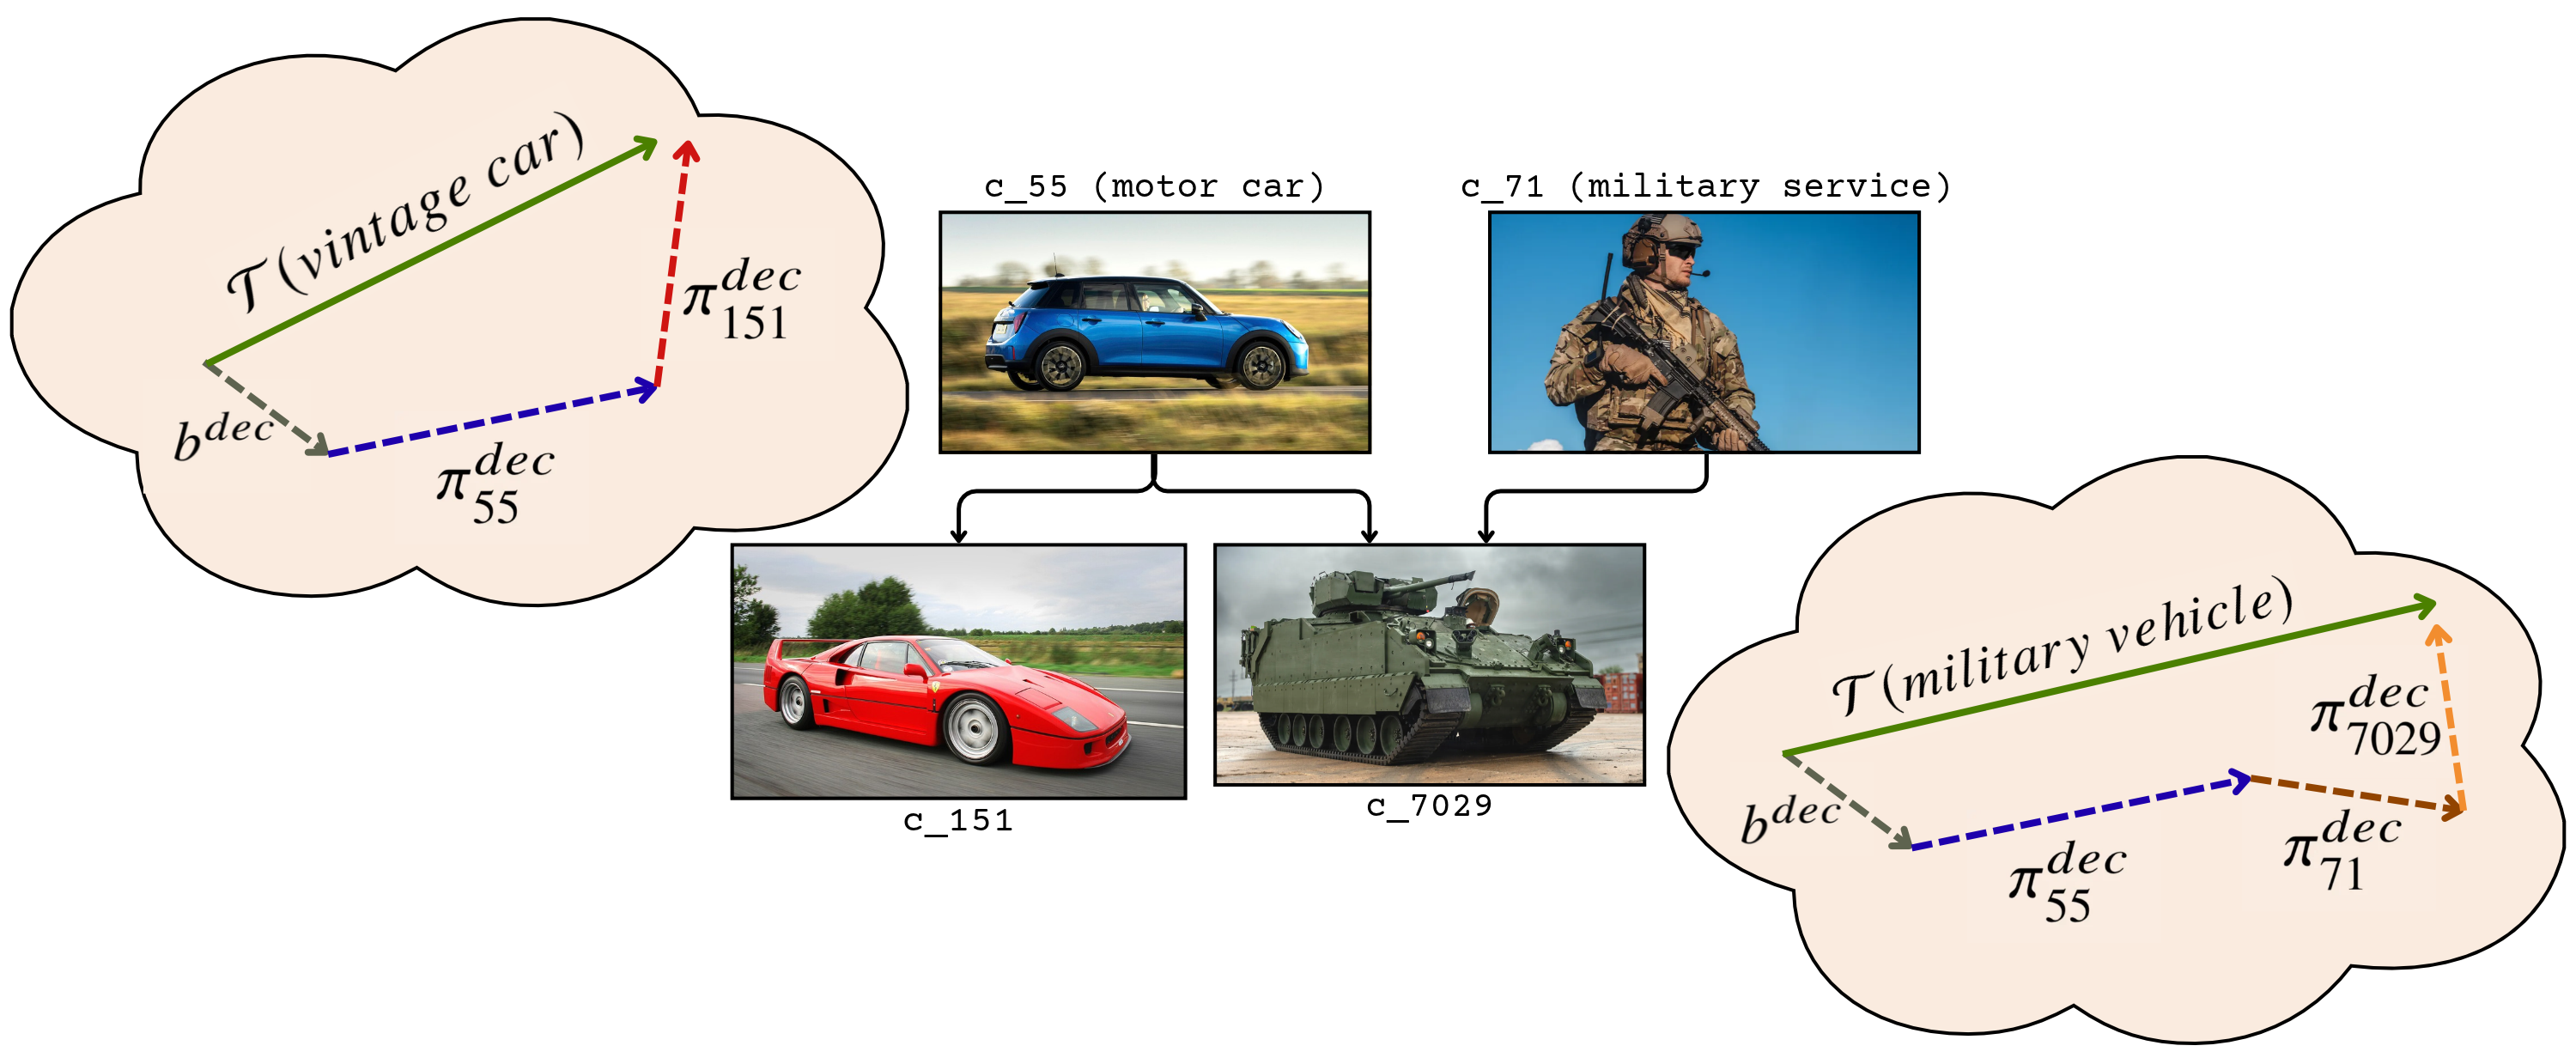
\includegraphics[width=0.65\linewidth]{naming.png}
    \end{figure}
\end{frame}

% -------------------------------------------------
\begin{frame}{CFM: from images to interpretable concepts}
    % \framesubtitle{METHOD}
    \begin{figure}
        \centering
        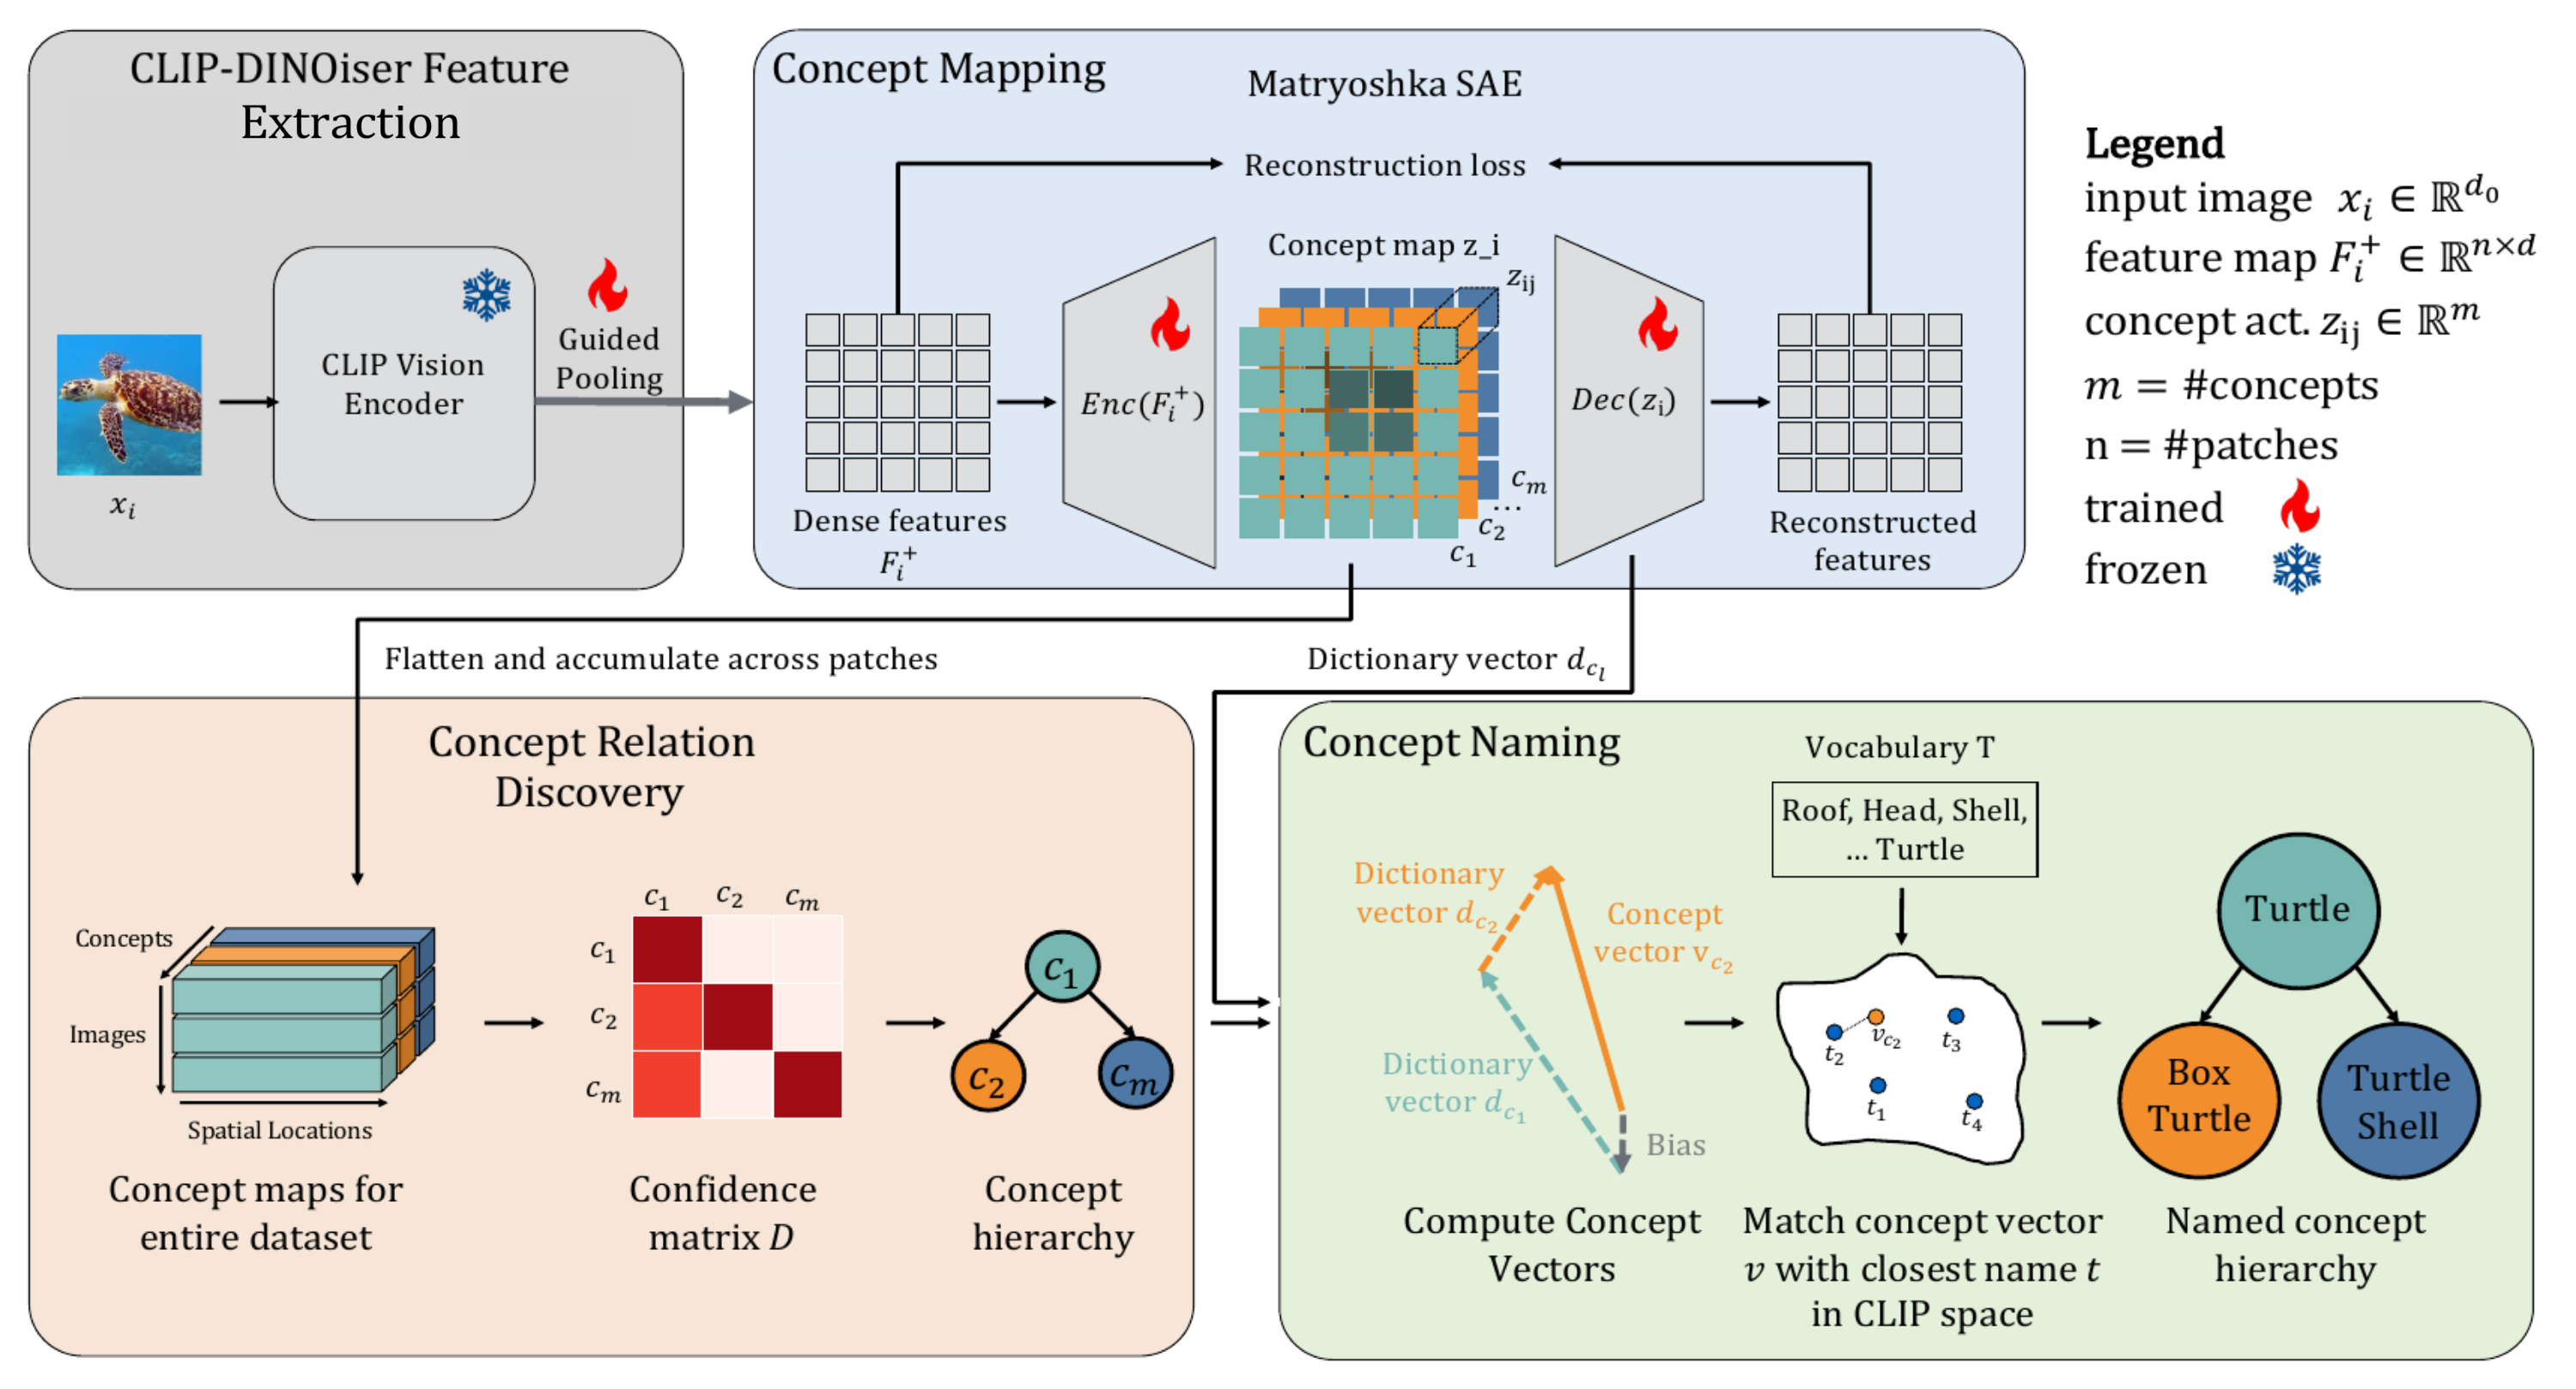
\includegraphics[width=0.8\linewidth]{method_summary.png}
    \end{figure}
\end{frame}

% -------------------------------------------------
\begin{frame}
\begin{center}
    \begin{minipage}{0.6\textwidth}
        \begin{block} {\centering \huge CFM Key Results}
            \begin{itemize}
                \item Improved Concept Quality and Naming
                \item Performance Across Downstream Tasks
                \item Steering through Concept-Level Intervention
            \end{itemize}
        \end{block}
    \end{minipage}
\end{center}
\end{frame}

% -------------------------------------------------
\begin{frame}{Improved Concept Quality}
    \framesubtitle{Comparison with previous approaches}

    \begin{columns}[T,onlytextwidth]
        \begin{column}{0.71\textwidth}
            \centering
            \scriptsize
            \textbf{Concept quality benchmarks}

            \vspace{0.3cm}

            \resizebox{\linewidth}{!}{
                \begin{tabular}{lrrrrrr}
                    \toprule
                    & \multicolumn{2}{c}{Locality $\uparrow$}
                    & \multicolumn{2}{c}{Consistency $\uparrow$}
                    & \multicolumn{2}{c}{Impurity $\downarrow$}\\
                    \cmidrule(lr){2-3}
                    \cmidrule(lr){4-5}
                    \cmidrule(lr){6-7}
                    Method & Part & Stuff & Part & Stuff & Part & Stuff\\
                    \midrule
                    SALF-CBM & 16.4 & 19.5 & 9.9 & 6.7 & .841 & 1.143\\
                    PatchSAE & 32.2 & 34.6 & 13.1 & 12.7 & .353 & .663\\
                    \textbf{CFM} & \textbf{44.3} & \textbf{44.5}
                    & \textbf{15.3} & \textbf{13.1}
                    & \textbf{.333} & \textbf{.539}\\
                    \bottomrule
                \end{tabular}
            }

            \vspace{0.4cm}

            {\scriptsize
            Part = PartImageNet; Stuff = COCO-Stuff.
            }

            % \vspace{0.2cm}
            \begin{center}
            \begin{minipage}{0.85\textwidth}
                \begin{block}{\small Main finding}
                \footnotesize
                CFM learns concepts that are more spatially localized,
                more consistent \\ and less impure than competing methods.
            \end{block}
            \end{minipage}
            \end{center}
        \end{column}

        \begin{column}{0.27\textwidth}
            \centering
            \scriptsize
            \textbf{Human Evaluation}

            \vspace{0.2cm}

            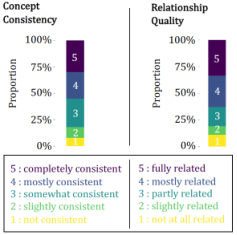
\includegraphics[
                width=\linewidth,
                height=0.46\textheight,
                keepaspectratio
            ]{figure3_user_study.png}

            \vspace{0.1cm}
            {\tiny  Fig. 3}

            \vspace{0.2cm}

            \scriptsize
            Human ratings of concept consistency
            and relationship quality.
        \end{column}
    \end{columns}
\end{frame}

% -------------------------------------------------
\begin{frame}{Concept Naming Accuracy}
    \framesubtitle{Do the assigned labels describe what is actually visible?}

    \begin{columns}[c,onlytextwidth]
        \begin{column}{0.35\textwidth}
            \centering
            {\Huge\bfseries +42.8}\par
            {\small percentage points}\par
            \vspace{0.15cm}
            \footnotesize
            Improvement in image-level concept-naming accuracy over a random baseline.

            \vspace{0.45cm}
            \begin{block}{\small Other methods}
                \footnotesize
                DN-CBM: +20.4 pp\\
                MSAE: +26.2 pp
            \end{block}
        \end{column}

        \begin{column}{0.62\textwidth}
            \centering
            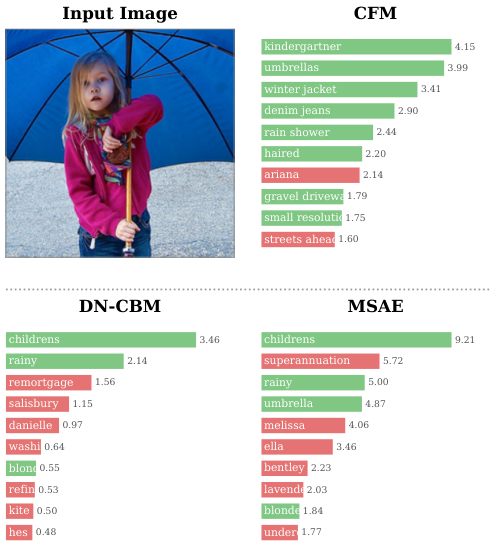
\includegraphics[
                width=\linewidth,
                height=0.58\textheight,
                keepaspectratio,
                trim=0 170bp 0 0,
                clip
            ]{figure5_naming.png}

            {\tiny Fig. 5: Green labels match visible content; red labels do not.}
        \end{column}
    \end{columns}

    \vfill
    \centering
    {\scriptsize Evaluation: top-10 concept names per image on COCO, judged by GPT-5-mini.}
\end{frame}

% -------------------------------------------------
\begin{frame}{Performance Across Downstream Tasks}
    \framesubtitle{What is the performance cost of interpretability?}

    \vspace{0.1cm}
    \centering
    \begin{tabular}{>{\raggedright\arraybackslash}p{0.53\linewidth}rr}
        \toprule
        \textbf{Task and metric} & \textbf{Opaque baseline} & \textbf{CFM} \\
        \midrule
        ImageNet, top-1 accuracy (\%) & 80.2 & 78.9 \\
        Places365, top-1 accuracy (\%) & 55.1 & \textbf{55.4} \\
        Open-vocabulary segmentation, mean mIoU & 41.4 & 41.3 \\
        Image captioning, CLIP-Score & 0.72 & 0.72 \\
        \bottomrule
    \end{tabular}

    \vspace{0.5cm}

    \begin{block}{\small Main finding}
        \centering
        CFM retains competitive performance while adding
        spatially grounded, interpretable concepts.
    \end{block}

    \vfill
    \begin{minipage}{0.95\linewidth}
        \tiny
        CLIP linear probe is the classification baseline; CLIP-DINOiser is used for
        segmentation and captioning. Fig. 6, Table 1, and Fig. 7.
    \end{minipage}
\end{frame}

% -------------------------------------------------
\begin{frame}{Steerable Image Captioning}
    \framesubtitle{Intervening on named concepts changes the generated caption}

    \centering
    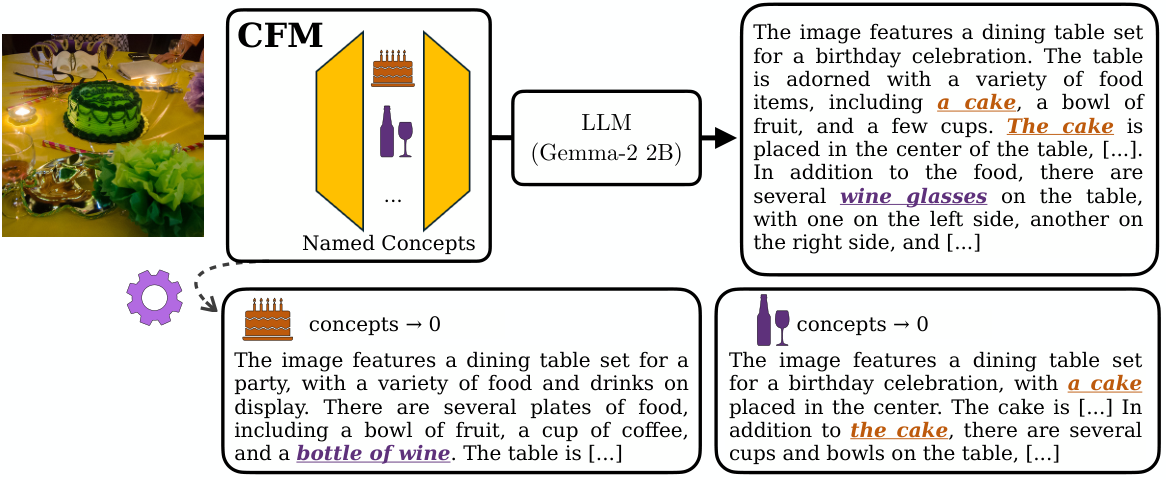
\includegraphics[
        width=0.96\linewidth,
        height=0.59\textheight,
        keepaspectratio
    ]{figure7_captioning.png}

    \vspace{0.08cm}
    {\tiny Fig. 7}

    \vspace{0.20cm}

    {\small Suppressing the \emph{cake} concept removes it from the caption,
    while suppressing the \emph{wine-glass} concept preserves the cake description.}
\end{frame}

% -------------------------------------------------
% Nie umieszczam faktu, ze hierarchiczne koncepty moga byc podatne
% na spurious correlation bo jest to wspomniane w paperze, ale najprawdopodobniej 
% wspomne o tym podczas mowienia o tym slajdzie
\begin{frame}{Critical Limitations}

    \begin{block}{Concept names are still imperfect}
        \small
        Some labels remain inaccurate or overly specific,
        even after hierarchy-aware naming.
    \end{block}

    \vspace{0.16cm}

    \uncover<2->{
        \begin{block}{Interpretability does not guarantee faithfulness}
            \small
            Spatially plausible concepts and successful interventions
            do not establish that every explanation captures the full causal basis
            of a prediction.
        \end{block}
    }

    \vspace{0.16cm}

    \uncover<3->{
        \begin{block}{Generalization needs broader testing}
            \small
            The reported experiments cover selected backbones, datasets,
            and tasks. Reliability under stronger distribution shifts
            remains an open question.
        \end{block}
    }

    \vfill
\end{frame}

% -------------------------------------------------
\begin{frame}{Discussion}

    \vspace{0.3cm}

    \begin{block}{Question 1:}
        \large
        Could CFM become for interpretable computer vision what CLIP became for vision-language understanding or SAM for segmentation?

        \vspace{0.15cm}
    \end{block}

    \vspace{0.5cm}

    \uncover<2->{
        \begin{block}{Question 2:}
            \large
            Are co-activation patterns sufficient to establish meaningful parent–child relationships between concepts?
        \end{block}
    }

\end{frame}

\end{document}
